\documentclass[10pt,aspectratio=43]{beamer}

\usetheme[sectionpages, logo={_figures/logo-federico-II-blue.pdf}]{UniNA}

\usepackage[utf8]{inputenc}
\usepackage[english]{babel}
\usepackage[T1]{fontenc}
\usepackage[scaled]{beramono}
\usepackage[scale=1.15]{AlegreyaSans}

\usepackage{csquotes}
\usepackage{biblatex}
\addbibresource{bibliography.bib}

\usepackage{amsmath}
\usepackage{booktabs}
\usepackage{graphicx}
\usepackage{listings}
\usepackage{caption}
\usepackage{subcaption}

\lstset{
    basicstyle=\ttfamily\scriptsize,
    keywordstyle=\color{blue}\bfseries,
    stringstyle=\color{red},
    commentstyle=\color{green!60!black},
    showstringspaces=false,
    breaklines=true,
    frame=single,
    rulecolor=\color{black!30},
    backgroundcolor=\color{gray!5}
}

\title[Kernel Batching with CUDA Graphs]{Kernel Batching with CUDA Graphs}
\subtitle{Replication Study and Performance Validation}
\author[Giuseppe Di Martino, Riccardo Regina]{Giuseppe Di Martino, Riccardo Regina}

\institute[
    Università degli Studi di Napoli Federico II
]
{
    Università degli Studi di Napoli Federico II
}

% \date{September 8, 2026}

\begin{document}

\maketitle

\begin{frame}{Agenda}{}
    \tableofcontents
\end{frame}

% ---------------------------------------------------------------
\section{Introduction}
% ---------------------------------------------------------------
\begin{frame}{Introduction}{Motivation and Context}
    \begin{itemize}
        \item \textbf{Goal}: Replicate and validate the findings of \textit{"Boosting Performance of Iterative Applications on GPUs: Kernel Batching with CUDA Graphs"} \cite{10974864} (PDP 2025).
        \item \textbf{Reproducibility}: Essential to verify robustness, ensure outcomes hold across architectures, and uncover implementation details.
        \item \textbf{The Problem}: GPU compute times are shrinking, but host-side kernel launch times remain steady.
        \item \textbf{Target Applications}: Iterative HPC applications (CFD, electromagnetic solvers, etc.) that execute the same sequences repeatedly.
        \item \textbf{The Solution}: NVIDIA introduced \textbf{CUDA Graphs}\footnote[frame]{\url{https://docs.nvidia.com/cuda/cuda-programming-guide/04-special-topics/cuda-graphs.html}} in CUDA 10 (2018) to move the scheduling burden to the device.
    \end{itemize}
\end{frame}

% ---------------------------------------------------------------
\section{CUDA Graphs}
% ---------------------------------------------------------------
\begin{frame}{CUDA Graphs}{A Paradigm Shift}
    \begin{block}{Traditional Execution}
        The host CPU dispatches operations sequentially to CUDA streams. When kernels are short-lived, CPU synchronization overhead can exceed GPU compute time.
    \end{block}
    
    \begin{block}{CUDA Graphs Execution}
        A directed acyclic graph (DAG) where nodes represent operations (kernels, memory copies) and edges denote dependencies.
        \begin{itemize}
            \item Exposes maximum inherent concurrency.
            \item Bypasses host CPU overhead.
        \end{itemize}
    \end{block}
\end{frame}

\begin{frame}{CUDA Graphs}{Lifecycle}
    The lifecycle of a CUDA Graph consists of three phases:
    \begin{enumerate}
        \item \textbf{Definition}: Constructing the topology (nodes and edges). Can be explicit (API calls) or implicit (stream capture). We focus on explicit creation for maximum control.
        \item \textbf{Instantiation}: Heavy-weight operation compiling the template into an executable format (\texttt{cudaGraphExec\_t}). Optimizes scheduling and pre-allocates resources. Done once.
        \item \textbf{Execution}: Launched repeatedly with a single API call (\texttt{cudaGraphLaunch}), bypassing per-kernel host overhead.
    \end{enumerate}
    \textit{Note:} For iterative apps, parameters (kernel args, grid dims) can be efficiently updated without destroying the instantiated graph.
\end{frame}

% ---------------------------------------------------------------
\section{The Unrolling Strategy}
% ---------------------------------------------------------------
\begin{frame}{The Unrolling Strategy}{Balancing Size and Overhead}
    \begin{itemize}
        \item \textbf{Too small}: A graph with 1-2 kernels yields negligible benefits.
        \item \textbf{Too big}: A graph spanning the entire application's lifespan incurs unsustainable creation overhead.
    \end{itemize}
    
    \begin{block}{The Mini-Batch Approach}
        Group a specific number of consecutive kernel launches into a localized subset: the \textbf{mini-batch} ($S$).
        \begin{itemize}
            \item Unrolled within a single static CUDA Graph.
            \item The main application loop iterates over this graph.
            \item Mirrors loop unrolling compiler optimizations.
        \end{itemize}
    \end{block}
\end{frame}

\begin{frame}{The Unrolling Strategy}{Visual Comparison}
    \begin{figure}
        \centering
        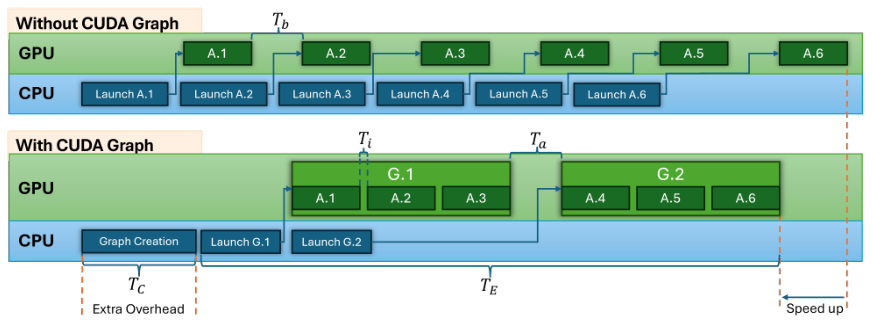
\includegraphics[width=\textwidth,height=0.4\textheight,keepaspectratio]{../article/figures/figure_1.pdf}
        \caption{Comparison between execution without CUDA graphs and the proposed unrolling strategy.}
    \end{figure}
    
    \begin{block}{Core Assumption}
        The strategy is fundamentally predicated on the assumption that \textbf{$T_i < T_a$}: the latency between kernels within the same graph ($T_i$) must be strictly lower than the launch overhead between independent graph executions ($T_a$).
    \end{block}
\end{frame}

% ---------------------------------------------------------------
\section{Performance Model}
% ---------------------------------------------------------------
\begin{frame}{Performance Model}{Overall and Creation Times}
    Overall execution time, $T$, is divided into graph creation time, $T_C$, and actual execution time, $T_E$:
    \begin{equation}
        T = T_C + T_E
    \end{equation}
    
    Given $I_k$ total kernel executions and a mini-batch size $S$, the number of iterations $I$ is:
    \begin{equation}
        I = \frac{I_k}{S}
    \end{equation}
    
    The graph creation time $T_C$ grows linearly with the mini-batch size $S$:
    \begin{equation}
        T_C = k_C \cdot S + b_C
    \end{equation}
    where $b_C$ is a fixed overhead and $k_C$ is the cost per node.
\end{frame}

\begin{frame}{Performance Model}{Execution Time Formulation}
    The actual execution time $T_E$ depends on the first graph launch time ($T_l$) and the time between independent graph executions ($T_a$):
    \begin{equation}
        T_{E} = T_{l} + T_{eg}\cdot I + T_{a}(I-1)
    \end{equation}
    
    The overall time of a single graph execution, $T_{eg}$, depends on a single kernel's execution time ($T_k$) and the time between kernels within the same graph ($T_i$):
    \begin{equation}
        T_{eg} = T_{k}S + T_{i}(S-1)
    \end{equation}
    
    Substituting the formulas yields:
    \begin{equation}
        T_E = \frac{I_{k}(T_{a}-T_{i})}{S} + I_{k}(T_{k} + T_{i}) - T_{a} + T_{l}
    \end{equation}
\end{frame}

\begin{frame}{Performance Model}{Simplified Execution Time}
    By isolating the constants, let:
    \begin{itemize}
        \item $a = I_{k}(T_{a}-T_{i})$
        \item $b = I_{k}(T_{k} + T_{i}) - T_{a} + T_{l}$
    \end{itemize}
    
    We can rewrite the execution time purely as a function of the mini-batch size $S$:
    \begin{equation}
        T_E = \frac{a}{S} + b
    \end{equation}
    
    \begin{itemize}
        \item $a$: The time gained between kernel executions by using CUDA Graphs.
        \item $b$: The lower bound on execution time (ignoring $-T_a + T_l$ for large $I_k$), effectively equivalent to one massive single graph.
    \end{itemize}
\end{frame}

\begin{frame}{Performance Model}{Vocabulary}
    \begin{table}
        \centering
        % \caption{Vocabulary of symbols used in the performance model.}
        \renewcommand{\arraystretch}{1.1}
        \resizebox{\columnwidth}{!}{%
        \begin{tabular}{lp{9cm}}
            \toprule
            \textbf{Symbol} & \textbf{Description} \\
            \midrule
            \(T\) & Overall execution time \\
            \(T_C\) & Graph creation time \\
            \(T_E\) & Actual execution time \\
            \(I_k\) & Total number of times the kernel must be executed \\
            \(S\) & Mini-batch size (number of nodes per graph) \\
            \(I\) & Total number of iterations (\(I_k / S\)) \\
            \(b_C\) & Fixed graph creation overhead \\
            \(k_C\) & Cost of creating a single graph node \\
            \(T_l\) & Launch time of the first graph execution \\
            \(T_{eg}\) & Overall execution time of a single graph \\
            \(T_a\) & Time between one graph execution and another \\
            \(T_k\) & Execution time of a single kernel \\
            \(T_i\) & Time between kernel executions within the same graph \\
            \bottomrule
        \end{tabular}%
        }
    \end{table}
\end{frame}

% ---------------------------------------------------------------
\section{Experimental Setup}
% ---------------------------------------------------------------
\begin{frame}{Experimental Setup}{Overview}
    To evaluate the proposed unrolling strategy, a custom CUDA application\footnote[frame]{\url{https://github.com/riccardoregina/CUDA-Graphs}} and a suite of test scripts were developed. 
    
    The entire experimental setup is divided into three main components:
    \begin{enumerate}
        \item \textbf{Core Skeleton Application}: A parameterizable C++/CUDA program to simulate iterative workloads.
        \item \textbf{Automation Scripts}: Bash scripts for batch execution, profiling, and data extraction.
        \item \textbf{Performance Modeling}: A curve fitting procedure to extract model coefficients and theoretical limits.
    \end{enumerate}
\end{frame}

\begin{frame}{Experimental Setup}{Skeleton Application}
    The custom CUDA application allows to test different configurations via CLI:
    \begin{itemize}
        \item \texttt{---num\_threads (-t)}: Total CUDA threads (grid dimension).
        \item \texttt{---inner\_iterations (-i)}: Iterations inside the kernel (increases arithmetic intensity).
        \item \texttt{---mini\_batch\_size (-k)}: Number of nodes in the graph ($S$).
        \item \texttt{---outer\_iterations (-o)}: Total times the graph/kernels are launched.
        \item \texttt{---repetitions (-r)}: Number of experiment repetitions for statistical robustness.
        \item \texttt{---seed (-s)}: Random seed for host memory init.
        \item \texttt{---use\_graph (-g)}: Toggle between standard streams (0) and CUDA Graphs (1).
    \end{itemize}
\end{frame}

\begin{frame}[fragile]{Experimental Setup}{Graph Creation Logic}
    \begin{figure}
\begin{lstlisting}[language=C++]
cudaGraphCreate(&graph, 0);
cudaGraphNode_t prev_node = nullptr;

for (int i = 0; i < mini_batch_size; ++i) {
    cudaGraphNode_t current_node;
    // ... set up kernelParams ...
    
    std::vector<cudaGraphNode_t> deps;
    if (prev_node != nullptr) {
        deps.push_back(prev_node);
    }
    
    cudaGraphAddKernelNode(&current_node, graph, 
                           deps.empty() ? nullptr : deps.data(), 
                           deps.size(), &kernelParams);
    prev_node = current_node;
}

cudaGraphInstantiate(&graphExec, graph, NULL, NULL, 0);
cudaGraphUpload(graphExec, 0);
\end{lstlisting}
        \caption{Core logic for creating and instantiating a CUDA Graph.}
    \end{figure}
\end{frame}

\begin{frame}{Experimental Setup}{Scripts}
    \begin{block}{Automation Scripts}
        \begin{itemize}
        \item \texttt{run\_increase\_nodes.sh}: measures the overhead of graph creation and execution depending on its size. It progressively increases the number of nodes (the mini-batch size) while keeping the total computational work constant, iterating across different thread counts to evaluate the scaling behavior.
        \item \texttt{run\_increase\_iterations.sh}: evaluates the overall speed-up provided by the unrolling strategy. Fixing the mini-batch size to an optimal value, it scales the number of total iterations and executes both the graph-enabled and the baseline versions of the application to gather comparative data.
        \item \texttt{profiler.sh}: instruments the application using NVIDIA Nsight Systems (\texttt{nsys}). It captures the hardware-level timeline of the GPU activity, crucial for verifying that the kernel batching and the graph dependencies are correctly enforced by the CUDA runtime.
        \end{itemize}
    \end{block}
\end{frame}
\begin{frame}{Experimental Setup}{Performance Modeling \& Curve Fitting}
    \begin{itemize}
        \item \textbf{Curve fitting} was performed on both graph creation and execution times against varying mini-batch sizes to validate the model.
        \item \textbf{Graph Execution Time ($T_E = a/S + b$)}: Fitting determines:
        \begin{itemize}
            \item $a$: Accumulated time gained between kernel executions.
            \item $b$: Theoretical lower bound of the execution time.
        \end{itemize}
        \item \textbf{Graph Creation Time ($T_C = k_C \cdot S + b_C$)}: Fitting identifies:
        \begin{itemize}
            \item $k_C$: Constant time cost per node.
            \item $b_C$: Fixed baseline creation overhead.
        \end{itemize}
    \end{itemize}
    
    \vspace{-0.1cm}
    \begin{block}{Optimal Batch Size ($S_{opt}$)}
        Extracting these constants allows to find the theoretical optimal batch size by minimizing the total time $T = T_C + T_E$:
        \begin{equation}
            \frac{dT}{dS} = k_C - \frac{a}{S^2} = 0 \implies S_{opt} = \sqrt{\frac{a}{k_C}}
        \end{equation}
    \end{block}
\end{frame}

\begin{frame}{Experimental Setup}{Hardware Configurations}
    Tested on three platforms, with GUI explicitly disabled via \texttt{systemctl isolate multi-user.target}:
    
    \begin{itemize}
        \item \textbf{Configuration A}: NVIDIA GeForce RTX 3070 (8 GB VRAM). \\Driver: 610.43.02, CUDA: 13.3.
        \item \textbf{Configuration B}: NVIDIA GeForce GTX 1060 (6 GB VRAM). \\Driver: 580.142, CUDA Toolkit: 12.6, Driver API: 13.0.
        \item \textbf{Configuration C}: NVIDIA Tesla T4 (16 GB VRAM). \\Driver: 580.82.07, CUDA: 13.0 (Google Colab).
    \end{itemize}
    
    \vspace{0.2cm}
    \textbf{Original Paper Baseline}: NVIDIA A100 (40 GB VRAM) with AMD EPYC 7302P host. \\Driver: 545.23.08, CUDA: 12.3.
\end{frame}

% ---------------------------------------------------------------
\section{Results}
% ---------------------------------------------------------------
\begin{frame}{Results}{Execution Trace Analysis}
    \begin{figure}
        \centering
        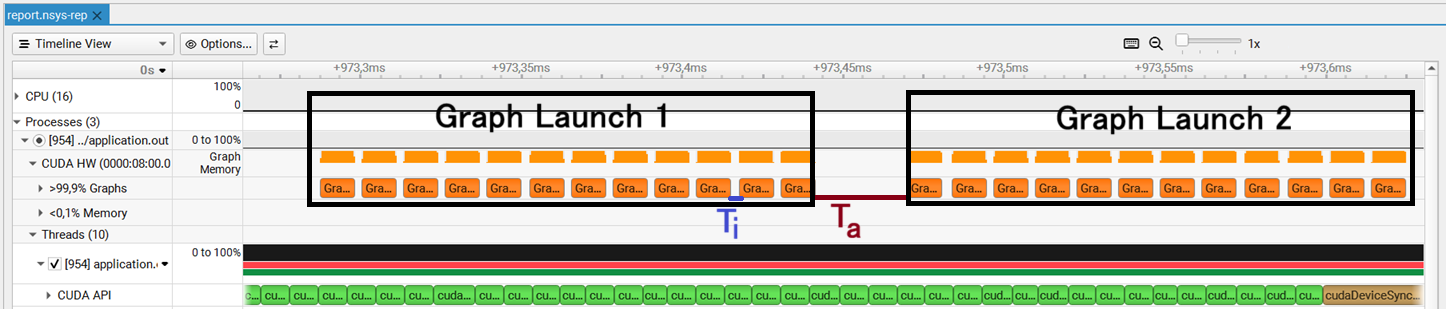
\includegraphics[width=\textwidth]{../article/figures/profiler.png}
        \caption{Execution trace from NVIDIA Nsight Systems. Visually confirms that launch overhead ($T_a$) is greater than inter-kernel latency ($T_i$).}
    \end{figure}
    Substantiates the core assumption $T_i < T_a$ explaining the time gain.
\end{frame}

\begin{frame}{Results}{Graph Creation Cost and Memory (RTX 3070)}
    \begin{figure}
        \centering
        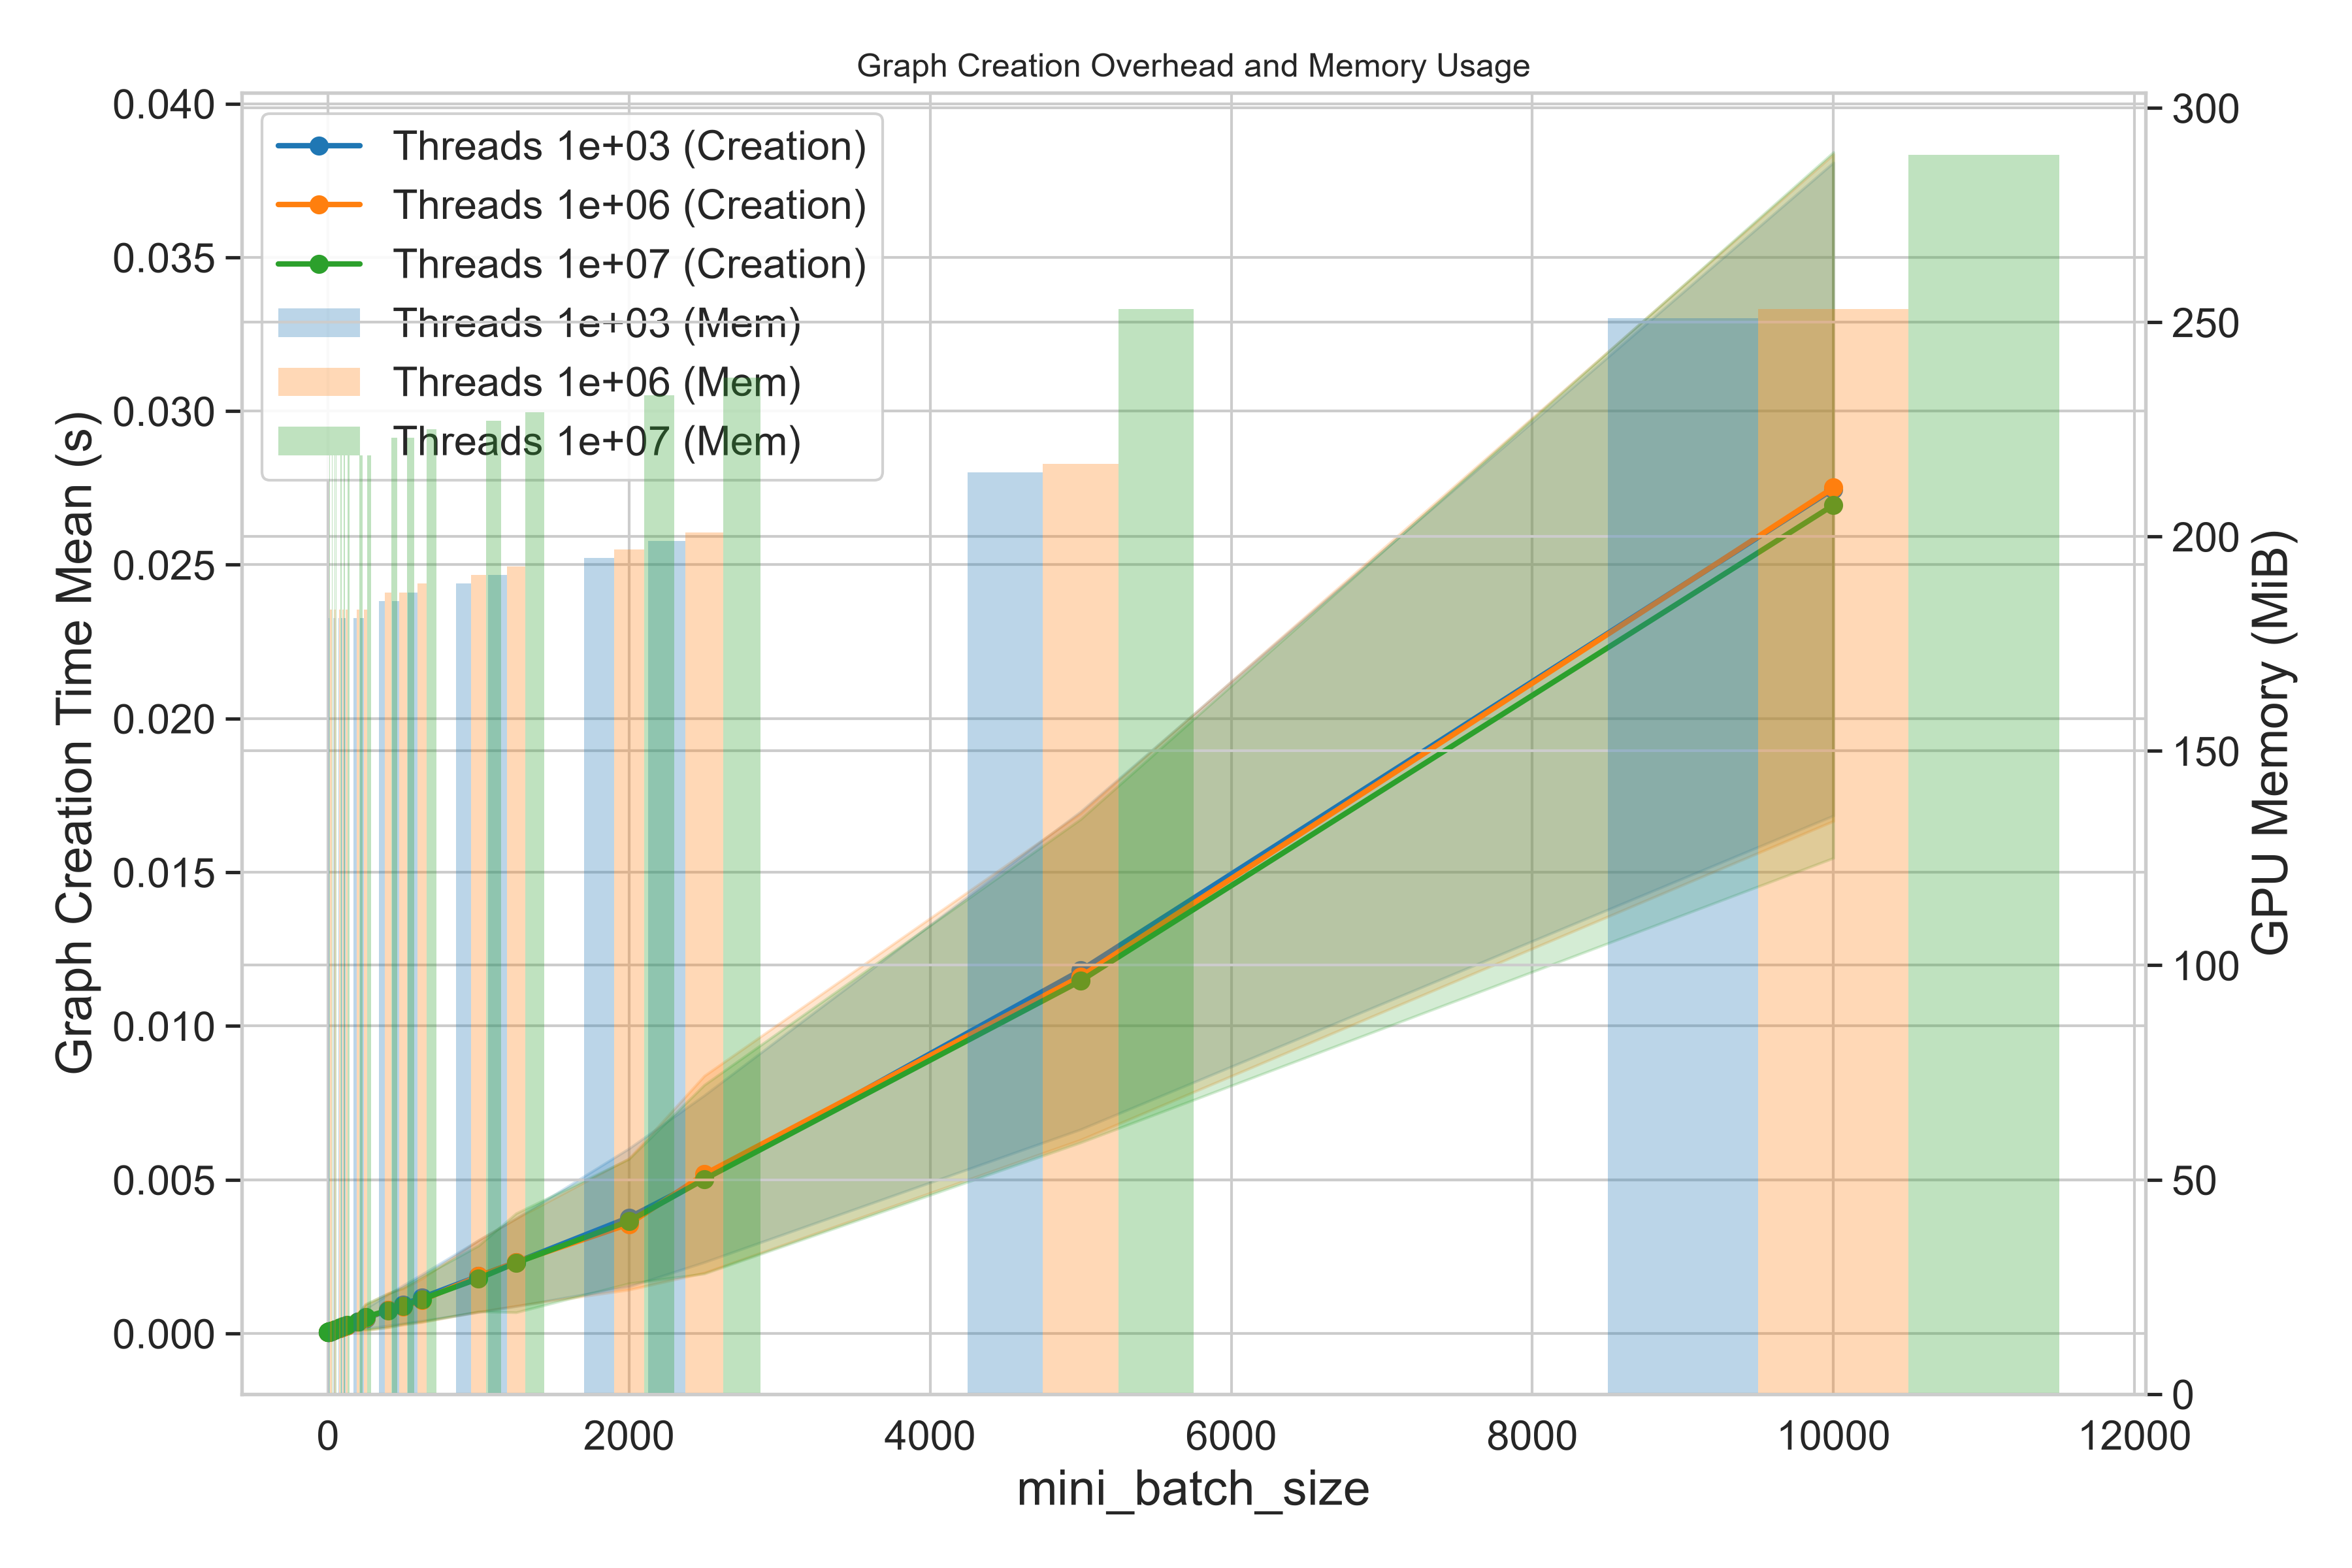
\includegraphics[height=0.7\textheight,width=\textwidth,keepaspectratio]{../assets/3070/figure_2.png}
        \caption{Creation Time and Memory for Config A (RTX 3070)}
    \end{figure}
\end{frame}

\begin{frame}{Results}{Graph Creation Cost and Memory (GTX 1060)}
    \begin{figure}
        \centering
        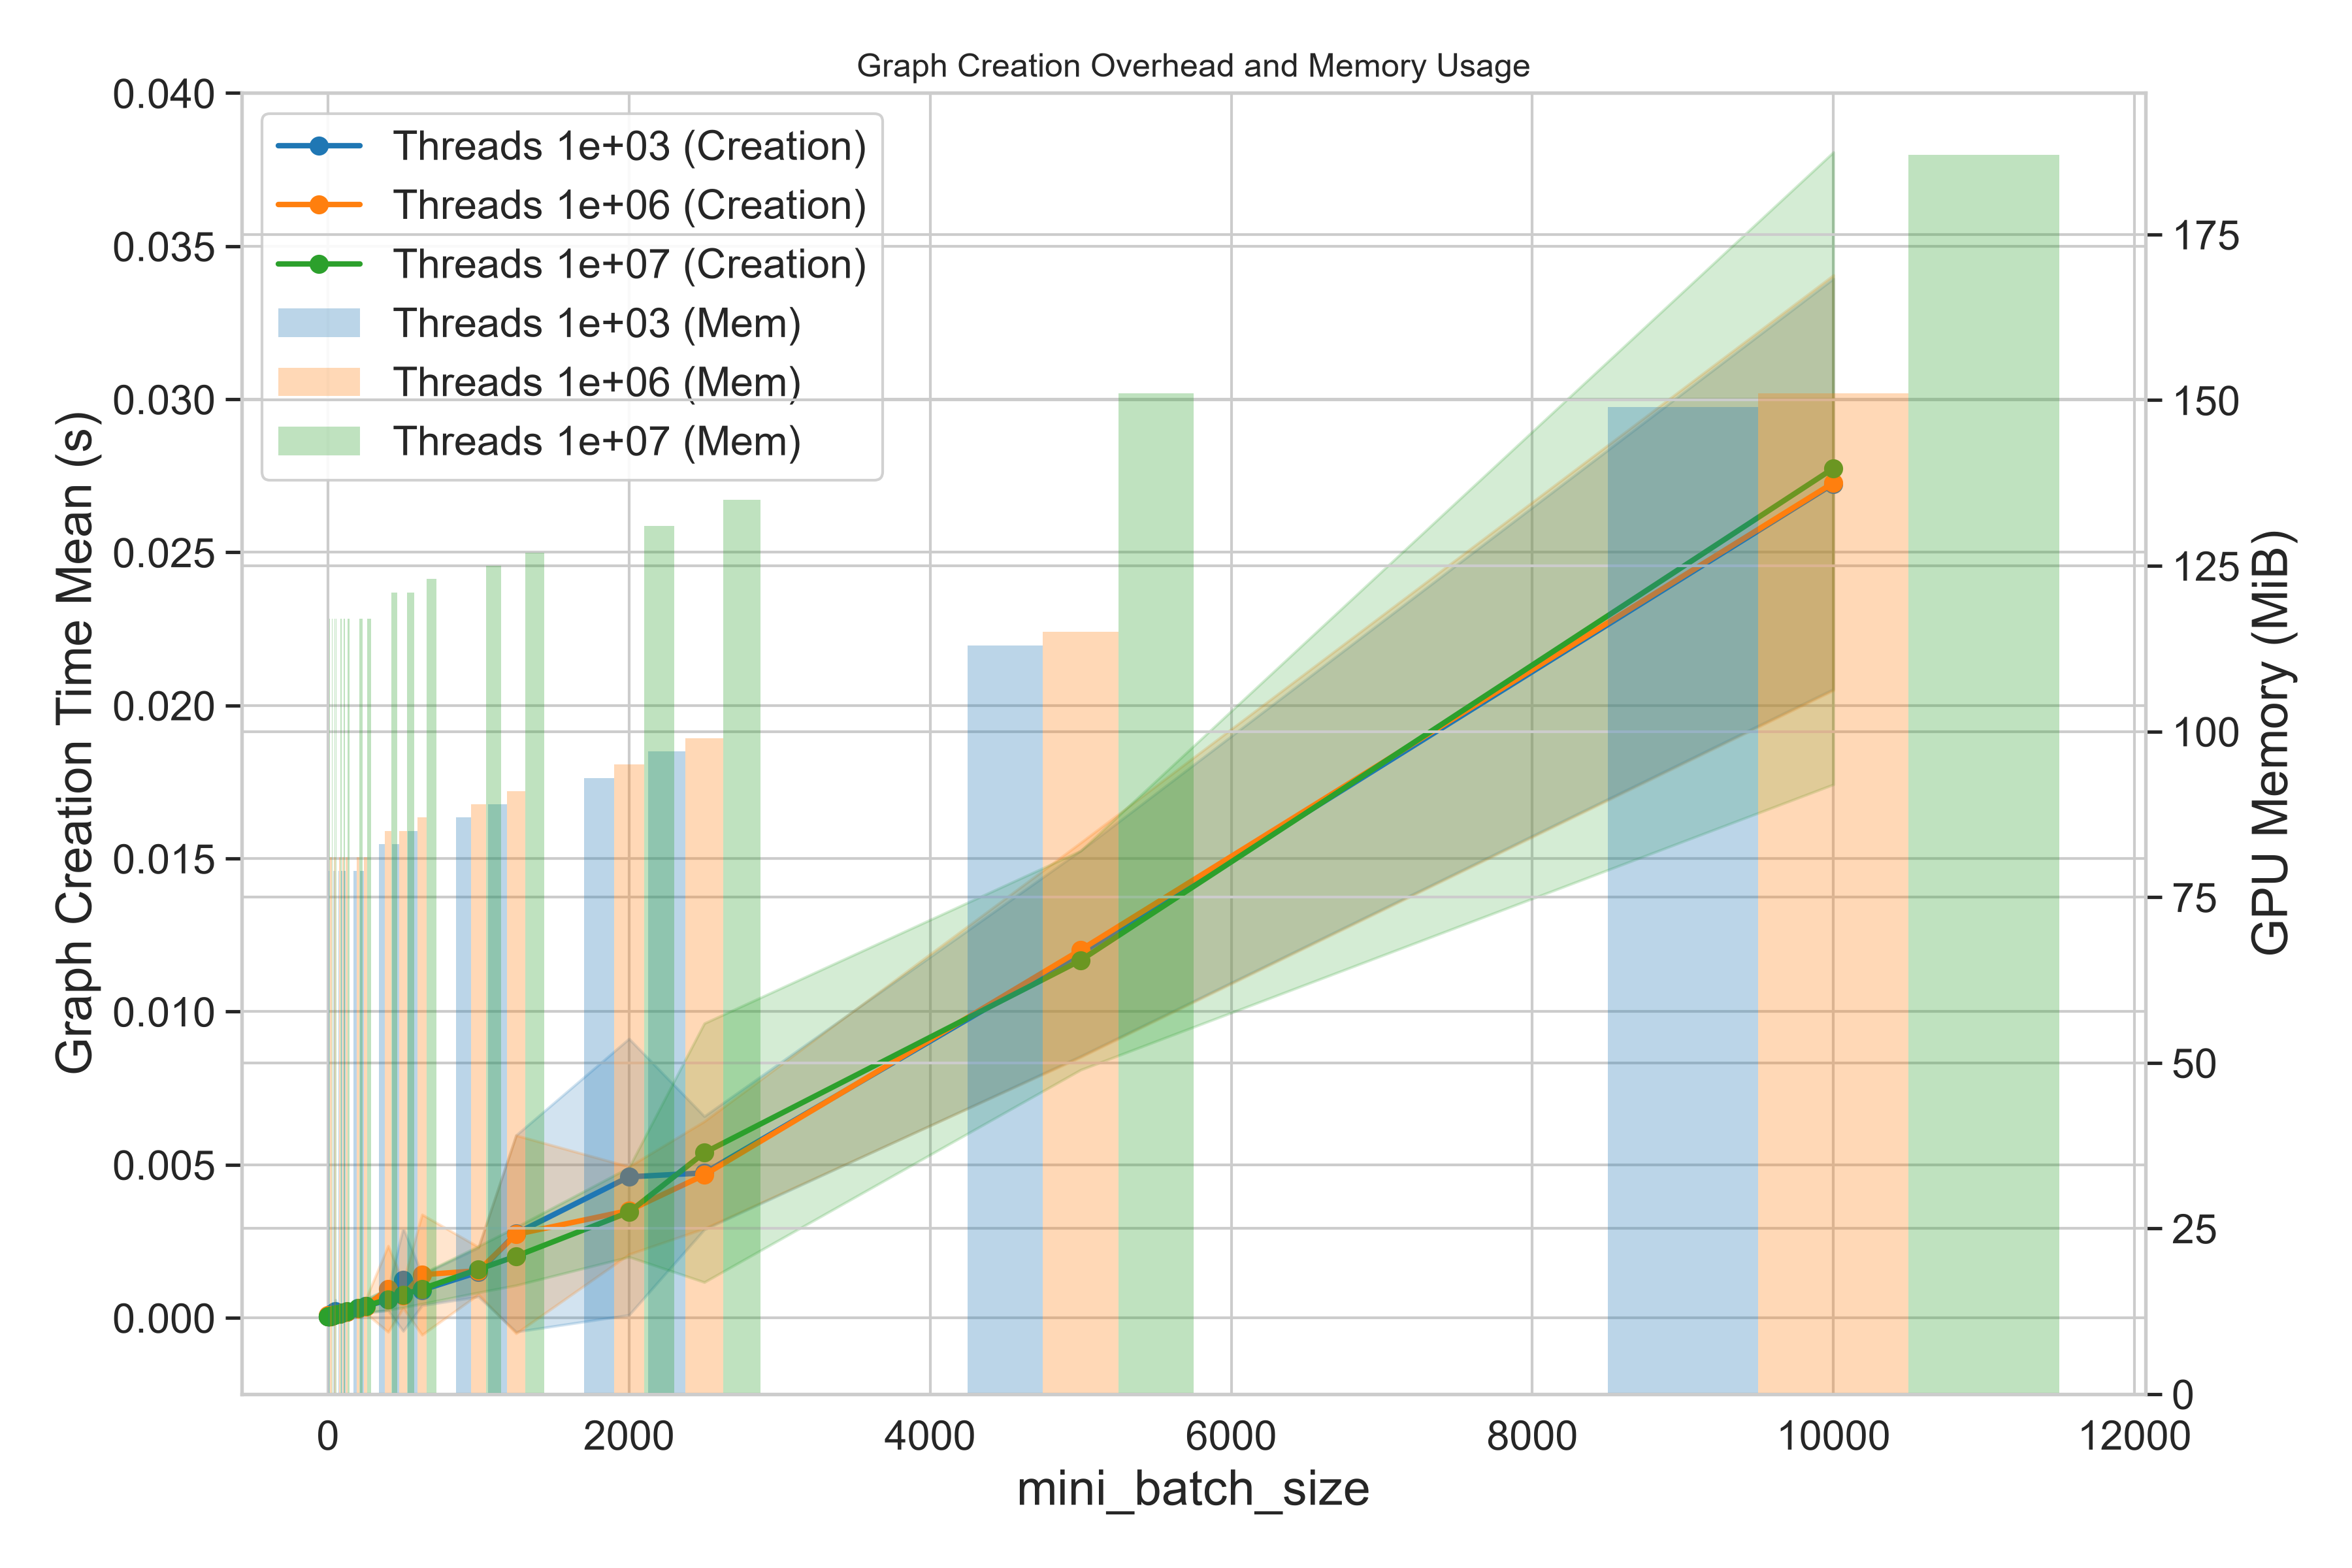
\includegraphics[height=0.7\textheight,width=\textwidth,keepaspectratio]{../assets/1060/figure_2.png}
        \caption{Creation Time and Memory for Config B (GTX 1060)}
    \end{figure}
\end{frame}

\begin{frame}{Results}{Graph Creation Cost and Memory (Tesla T4)}
    \begin{figure}
        \centering
        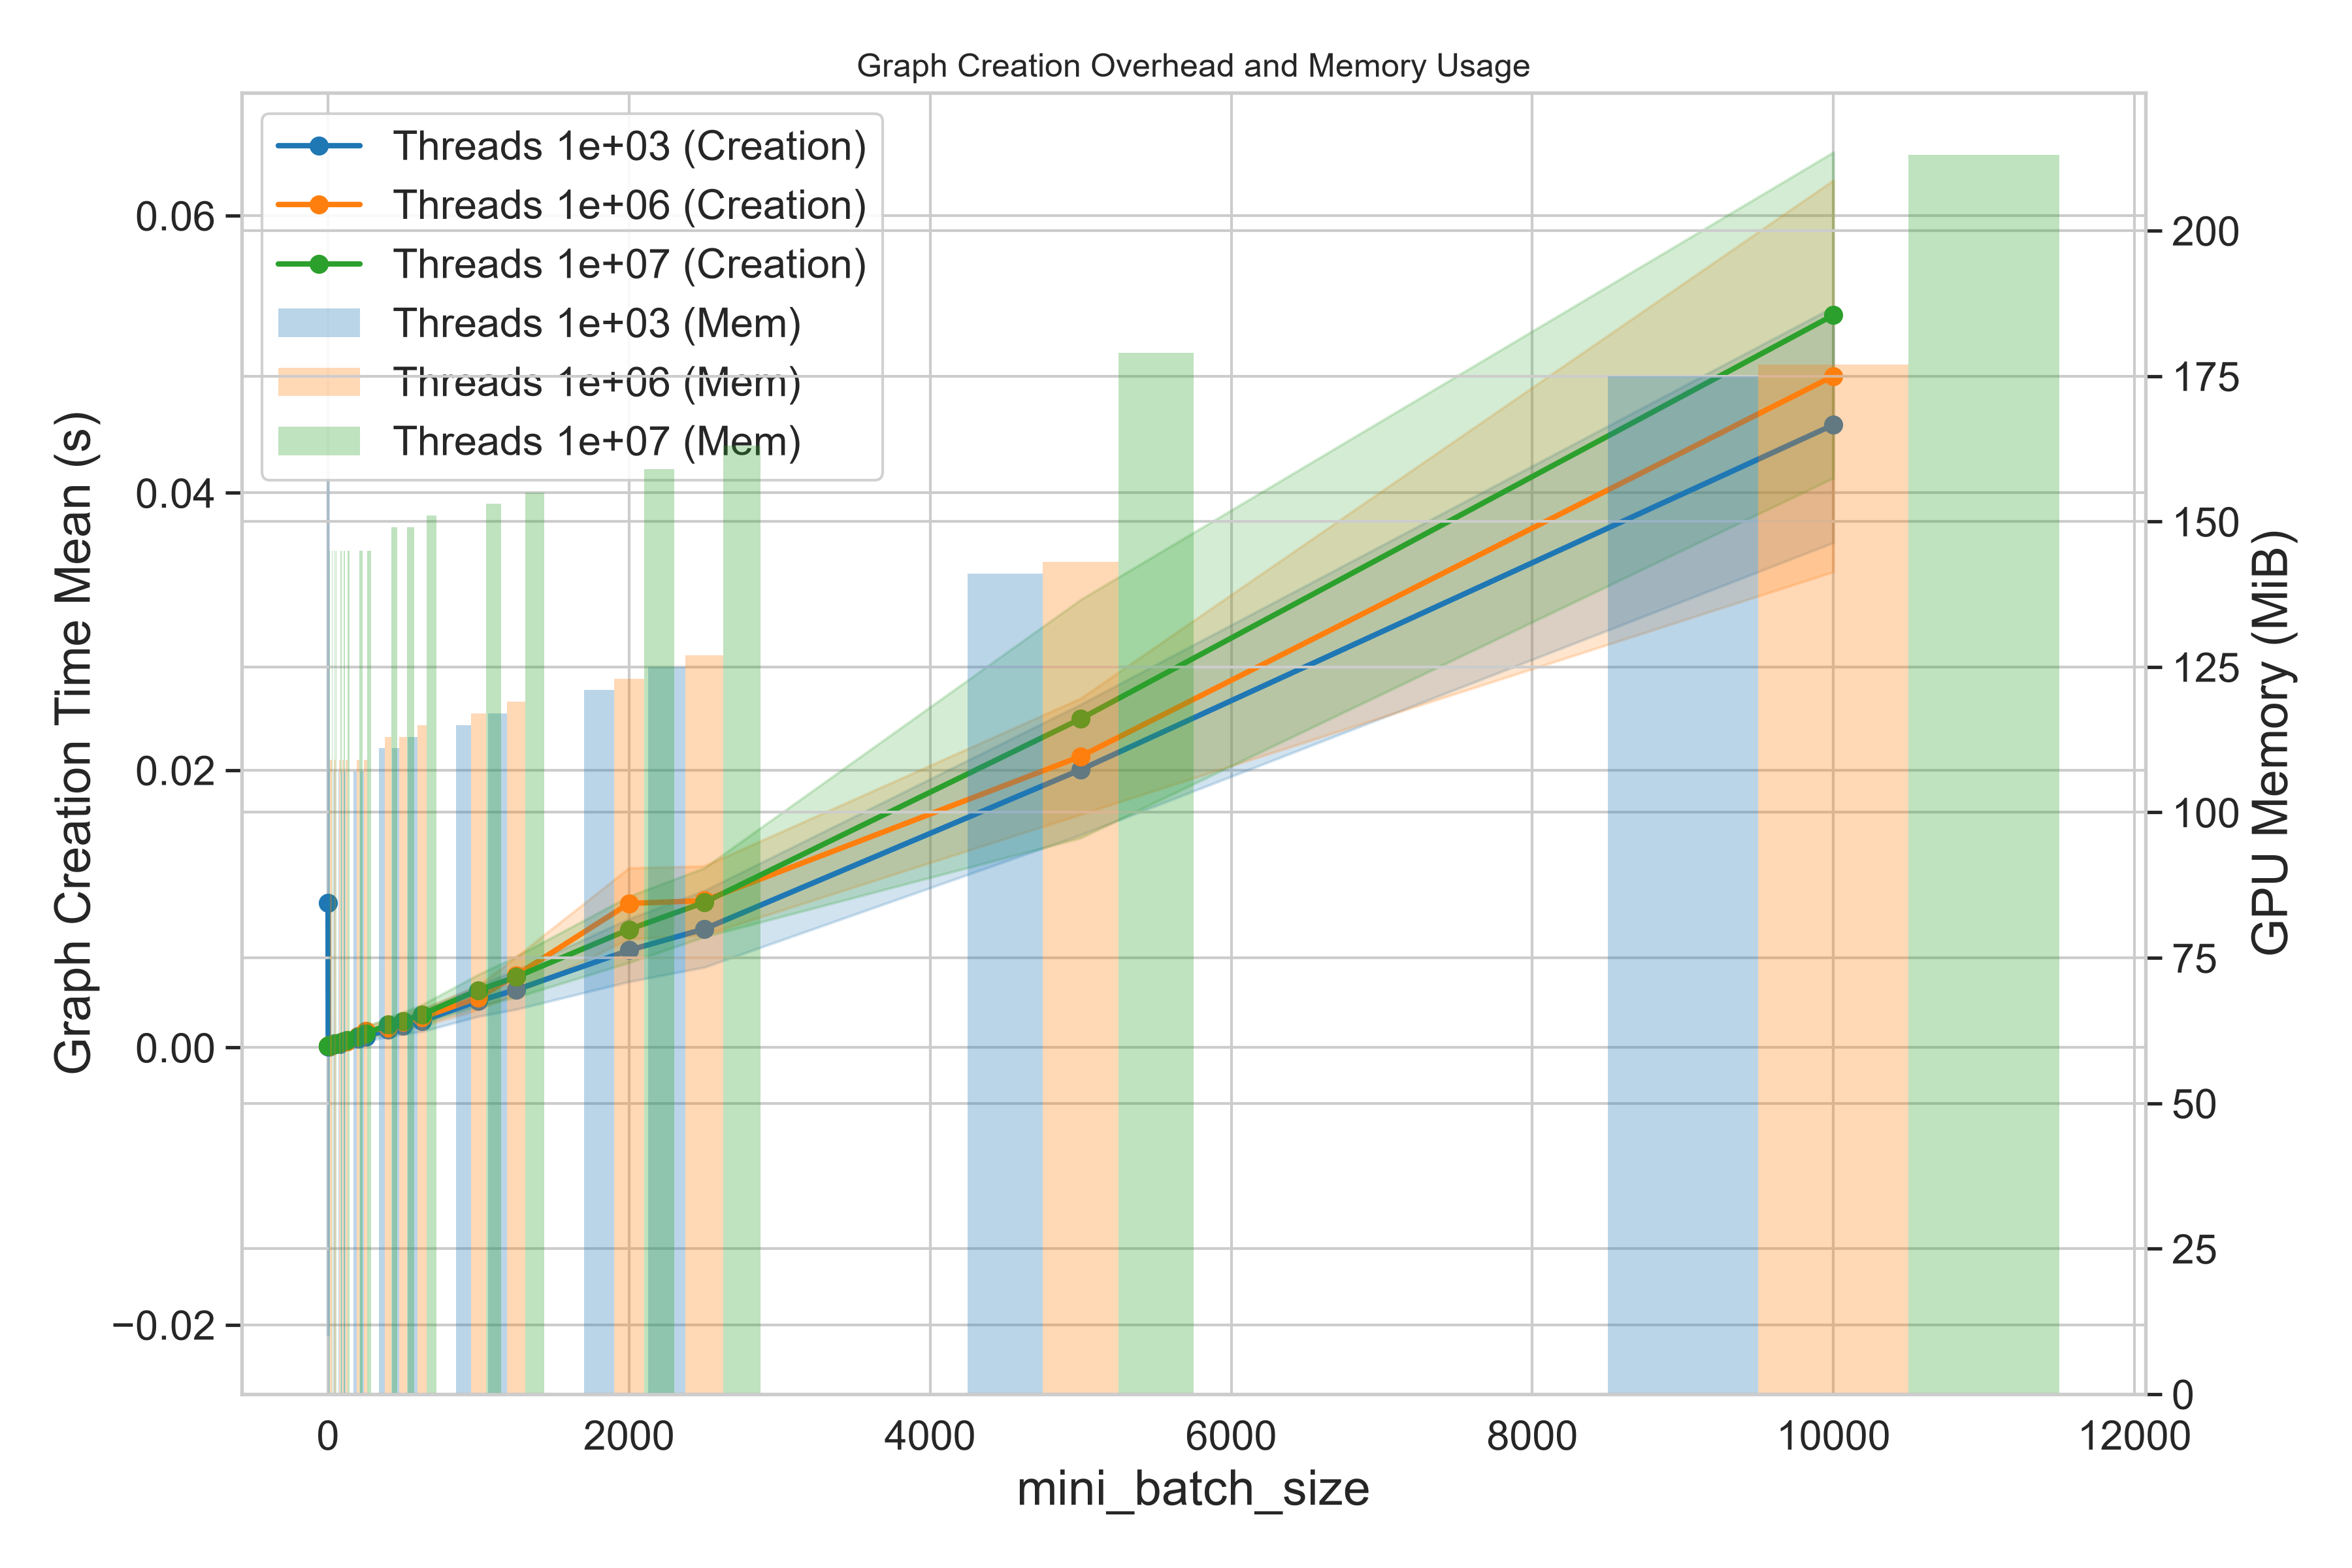
\includegraphics[height=0.7\textheight,width=\textwidth,keepaspectratio]{../assets/t4/figure_2.png}
        \caption{Creation Time and Memory for Config C (Tesla T4)}
    \end{figure}
\end{frame}

\begin{frame}{Results}{Graph Creation Cost and Memory (Original Paper)}
    \begin{figure}
        \centering
        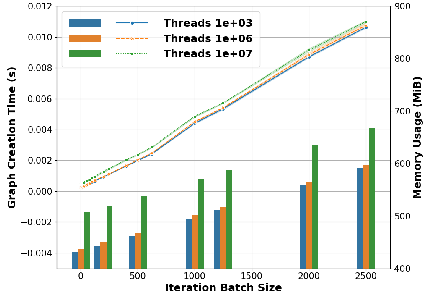
\includegraphics[height=0.7\textheight,width=\textwidth,keepaspectratio]{../article/figures/figure_2.pdf}
        \caption{Creation Time and Memory (Original Results)}
    \end{figure}
\end{frame}

\begin{frame}{Results}{Graph Creation Cost and Memory Insights}
    \begin{itemize}
        \item Linearity maintained up to \textbf{10,000 nodes} (vs 2,500 in original paper).
        \item Memory footprint is lower: \textbf{~300 MiB} at 10,000 nodes (vs 700-800 MiB at 2,500 nodes).
    \end{itemize}
\end{frame}

\begin{frame}{Results}{Creation Time Fitting (RTX 3070)}
    \begin{table}
        \centering
        \caption{Fitting parameters for Graph Creation Time ($T_C = a \cdot S + b$)}
        \renewcommand{\arraystretch}{1.2}
        \begin{tabular}{rccc}
            \toprule
            \textbf{Workload} & \textbf{\(a\)} & \textbf{\(b\)} & \textbf{MAE} \\
            \midrule
            \(10^3\) & $2.64 \times 10^{-6}$ & $-2.70 \times 10^{-4}$ & $4.23 \times 10^{-4}$ \\
            \(10^6\) & $2.64 \times 10^{-6}$ & $-2.76 \times 10^{-4}$ & $4.49 \times 10^{-4}$ \\
            \(10^7\) & $2.59 \times 10^{-6}$ & $-2.56 \times 10^{-4}$ & $4.28 \times 10^{-4}$ \\
            \bottomrule
        \end{tabular}
    \end{table}
    
    \textit{Note: For Config C (Tesla T4), creation time increases slightly with workload due to upload overhead, confirming the original paper. Config A and B are independent of workload.}
\end{frame}

\begin{frame}{Results}{Graph Execution Time (RTX 3070)}
    \begin{figure}
        \centering
        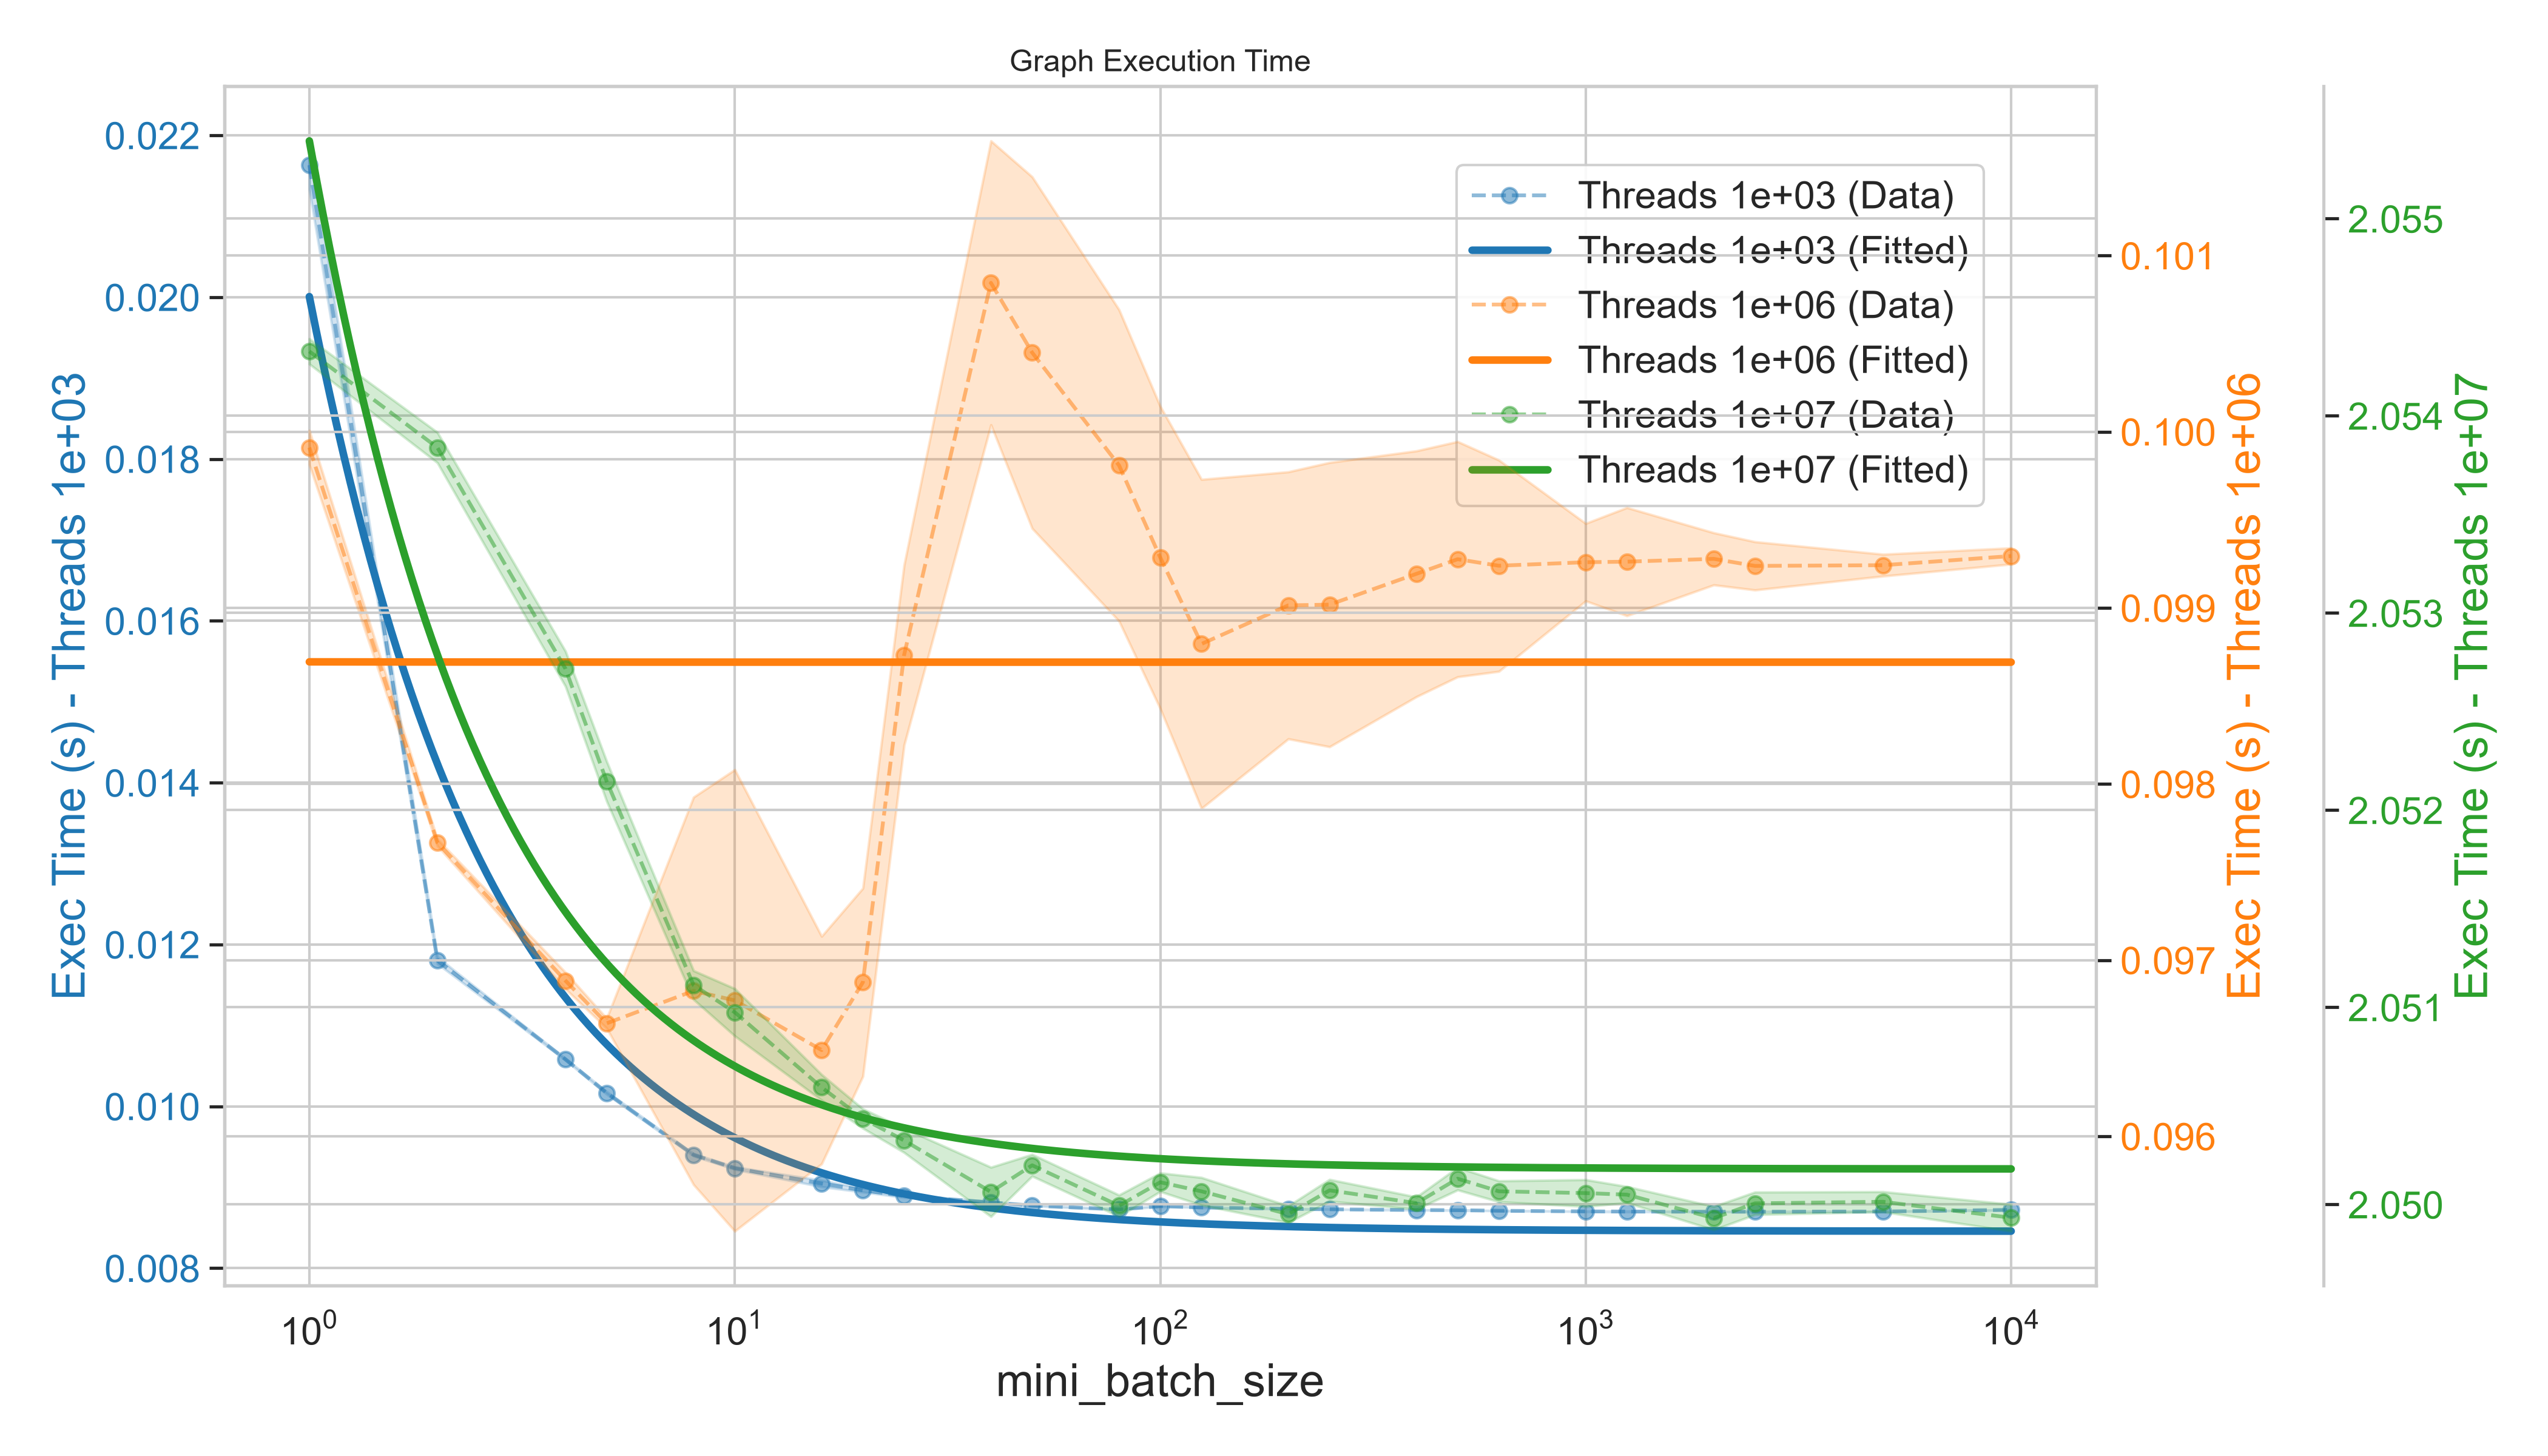
\includegraphics[height=0.7\textheight,width=\textwidth,keepaspectratio]{../assets/3070/figure_3.png}
        \caption{Graph Execution Time for Config A (RTX 3070)}
    \end{figure}
\end{frame}

\begin{frame}{Results}{Graph Execution Time (GTX 1060)}
    \begin{figure}
        \centering
        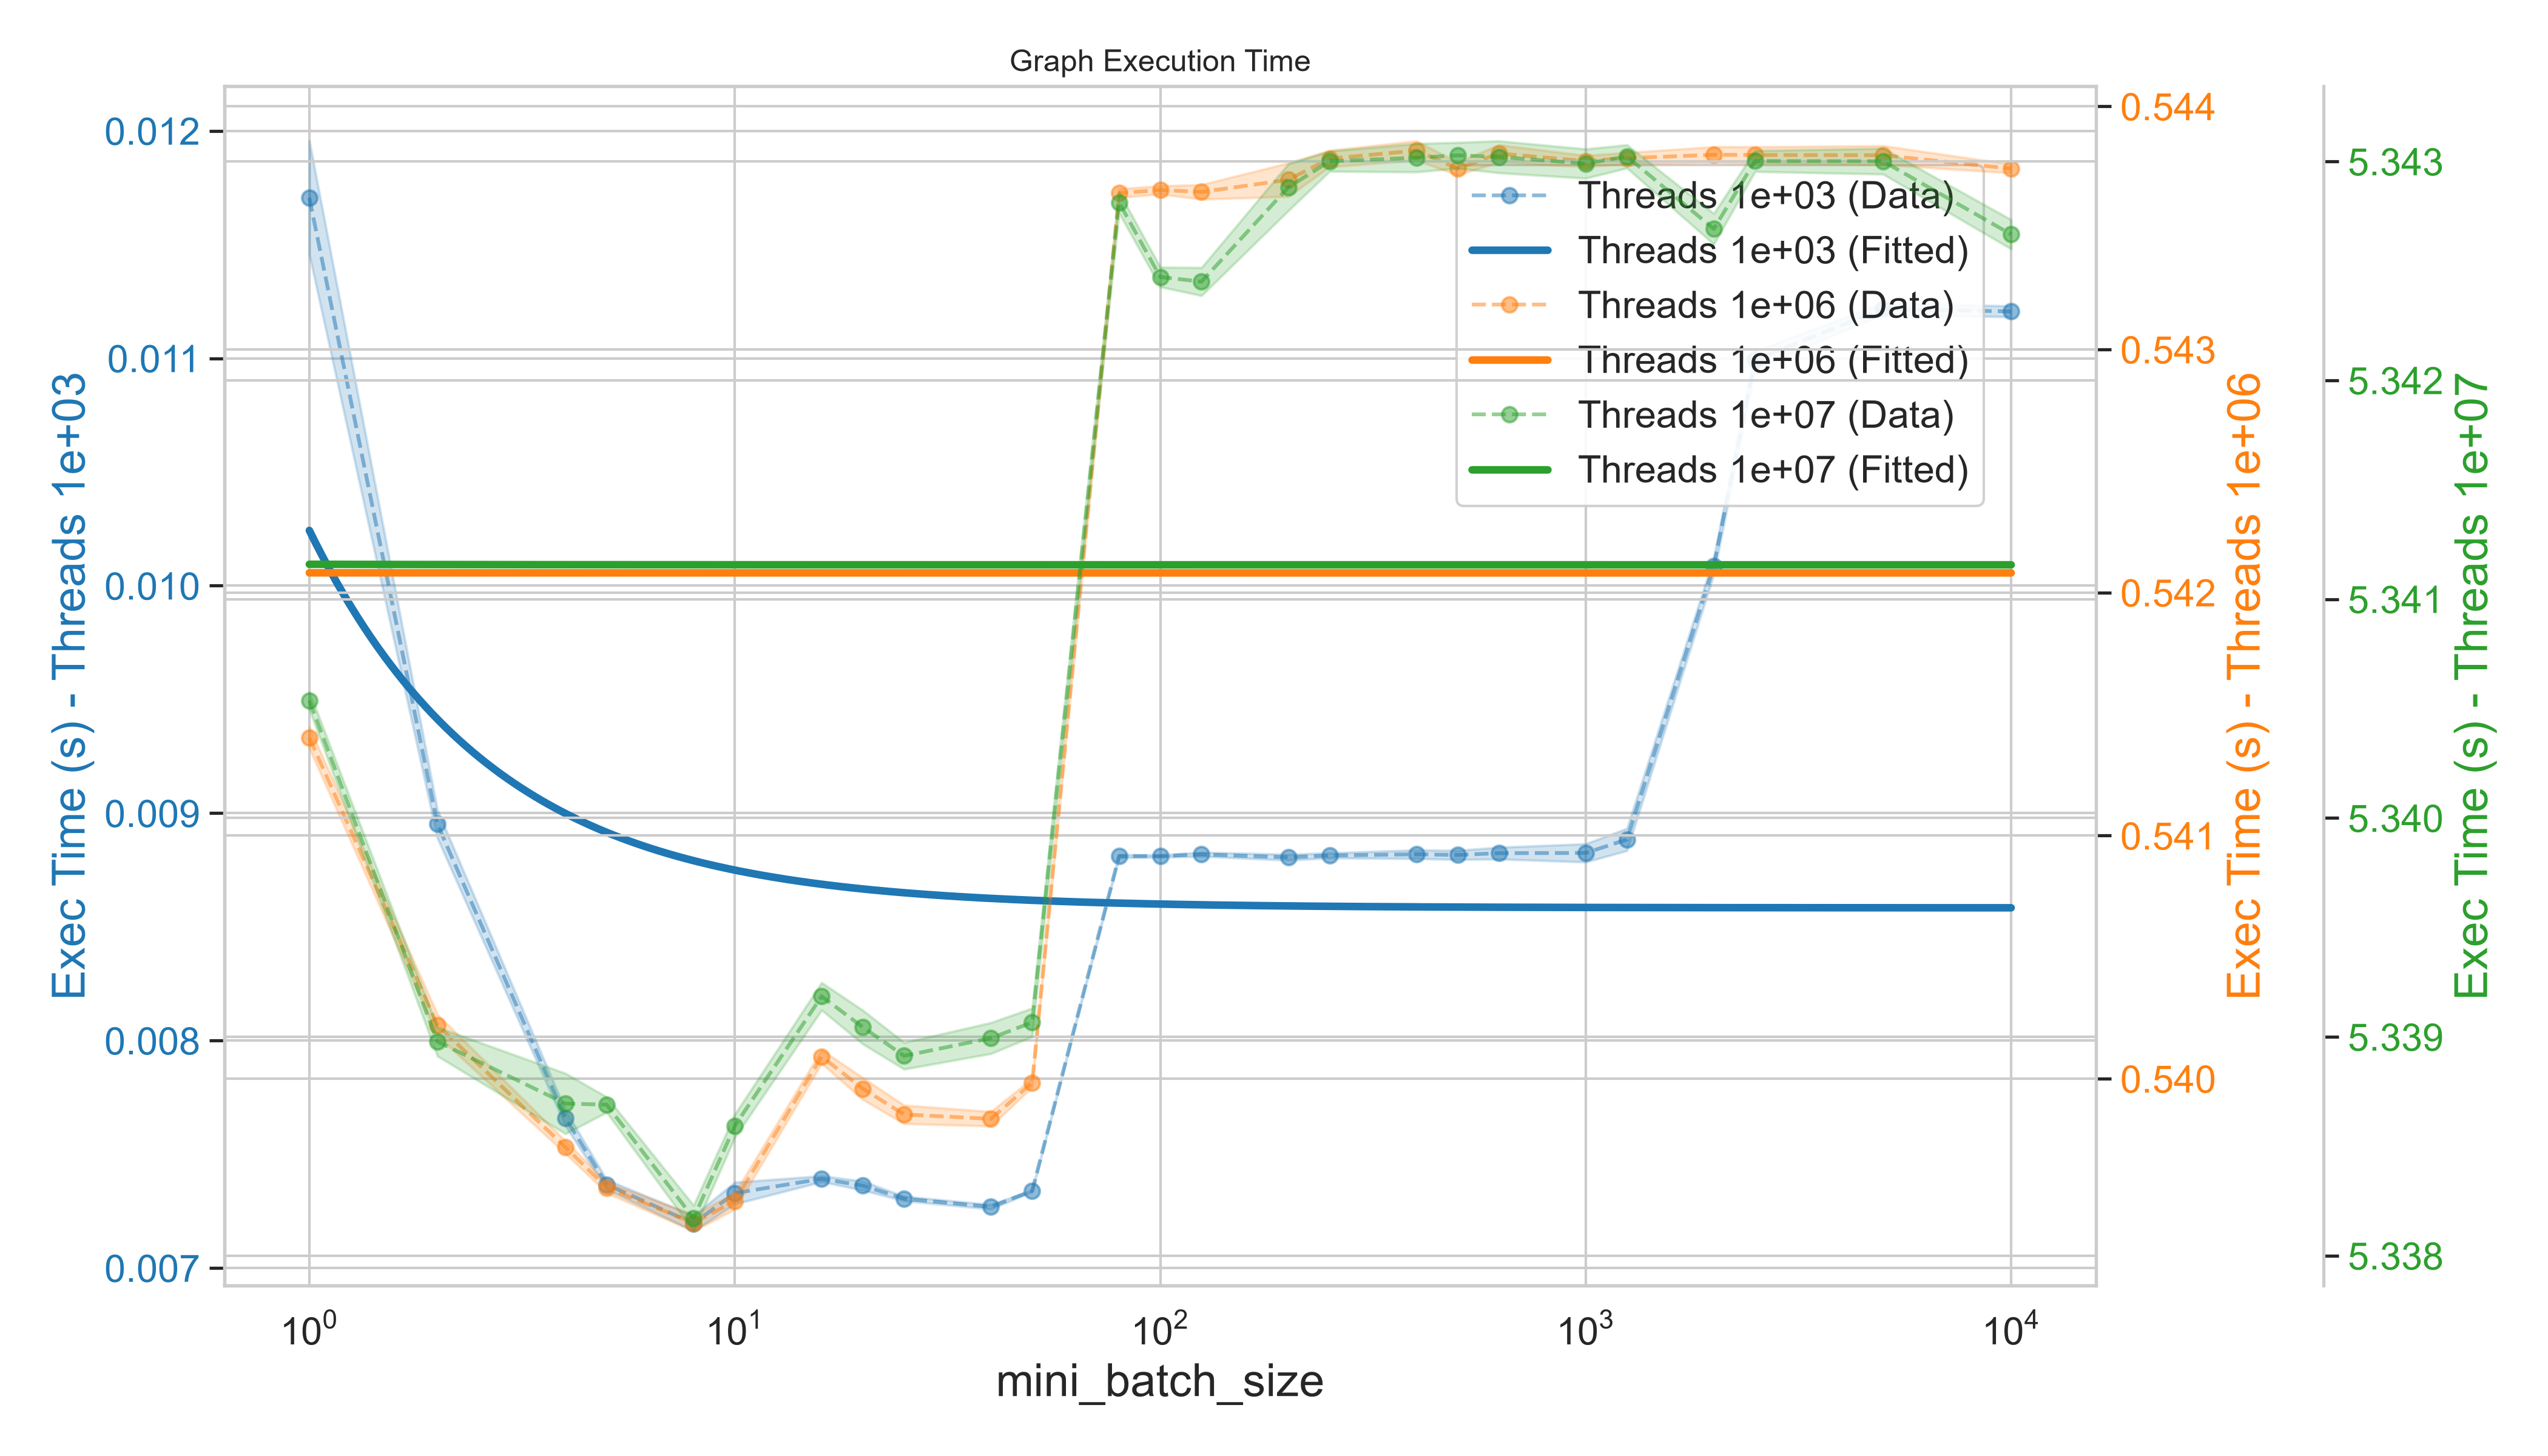
\includegraphics[height=0.7\textheight,width=\textwidth,keepaspectratio]{../assets/1060/figure_3.png}
        \caption{Graph Execution Time for Config B (GTX 1060)}
    \end{figure}
\end{frame}

\begin{frame}{Results}{Graph Execution Time (Tesla T4)}
    \begin{figure}
        \centering
        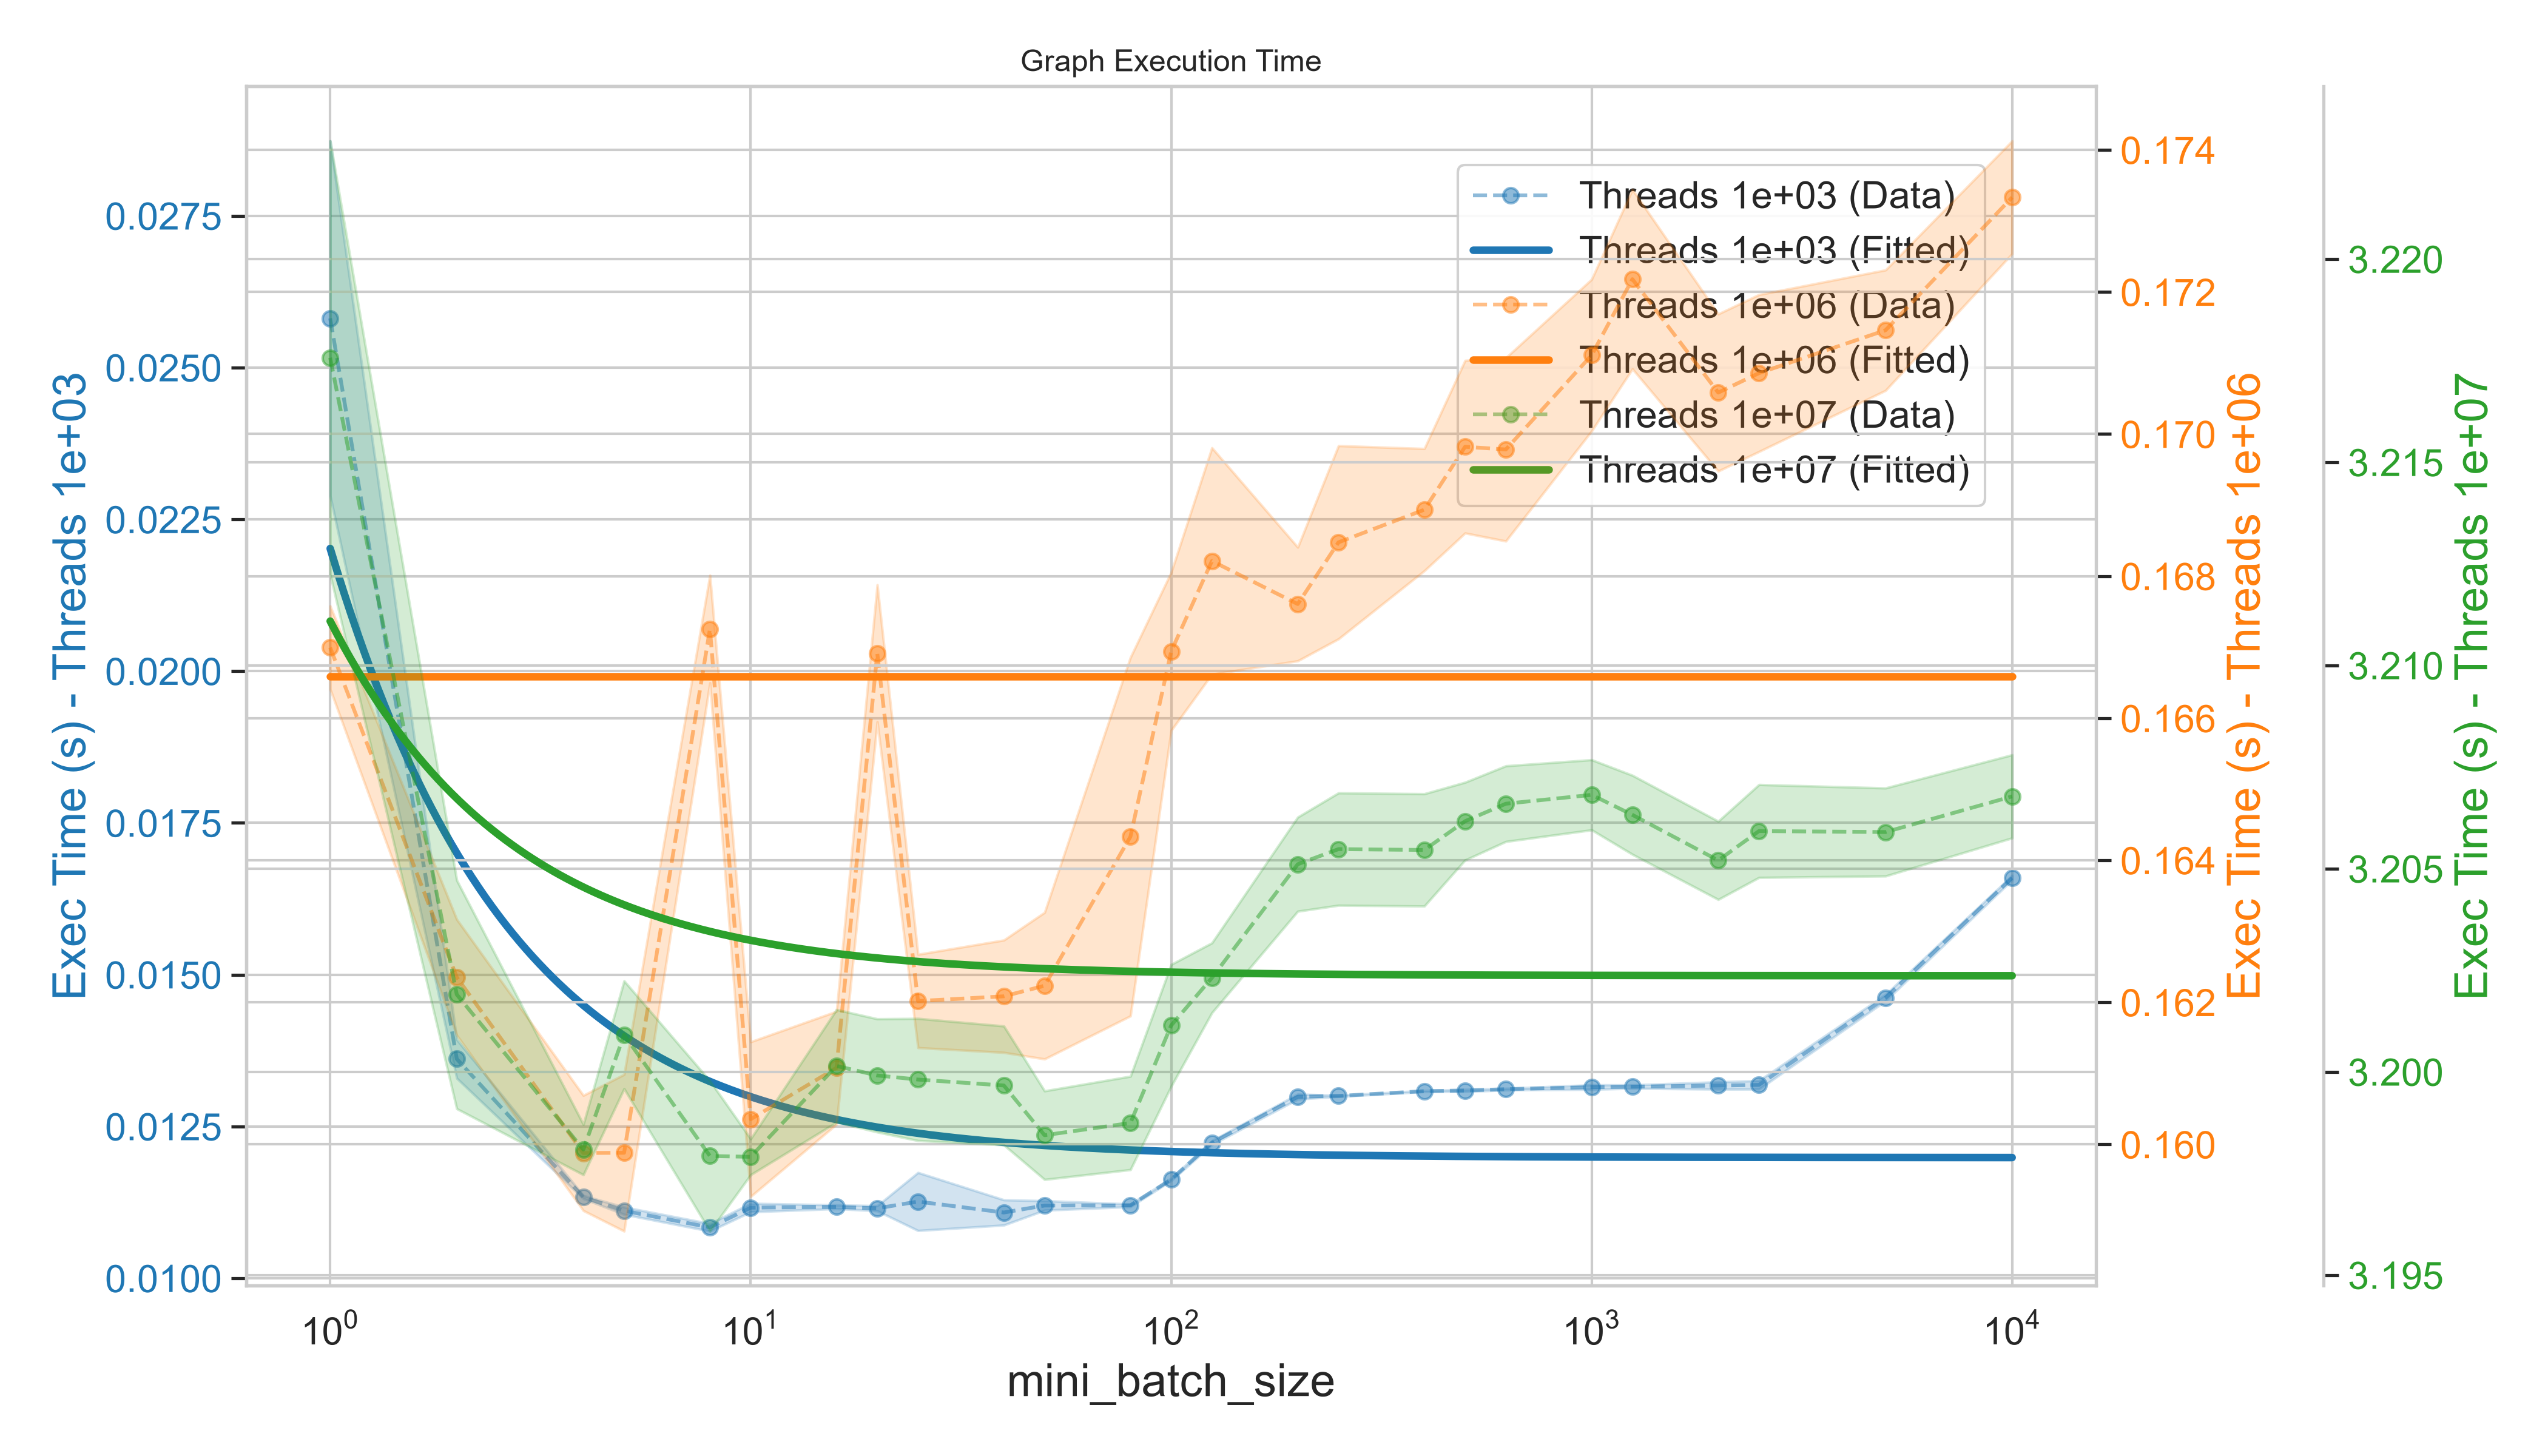
\includegraphics[height=0.7\textheight,width=\textwidth,keepaspectratio]{../assets/t4/figure_3.png}
        \caption{Graph Execution Time for Config C (Tesla T4)}
    \end{figure}
\end{frame}

\begin{frame}{Results}{Graph Execution Time (Original Paper)}
    \begin{figure}
        \centering
        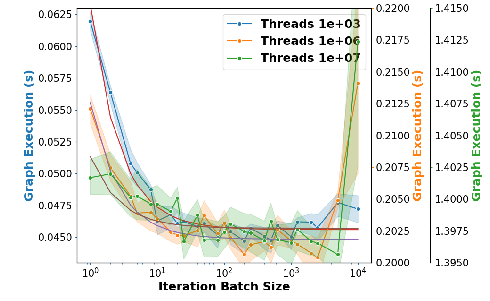
\includegraphics[height=0.7\textheight,width=\textwidth,keepaspectratio]{../article/figures/figure_3.pdf}
        \caption{Graph Execution Time (Original Results)}
    \end{figure}
\end{frame}

\begin{frame}{Results}{Execution Time Insights}
    \begin{itemize}
        \item Model predicts execution time converges to a lower asymptote.
        \item \textbf{Spike at $10^6$ threads}: Between 30 and 100 batch size, performance degrades. \textbf{Not observed on A100} in the original paper. We attribute this to \textbf{L2 cache saturation} on our GPUs with smaller caches, causing memory latencies.
        \item \textbf{Resilience at scale}: Execution times remain stable up to 10,000 nodes, unlike original paper which noted resource exhaustion past 2,500 nodes.
    \end{itemize}
    
    \begin{table}
        \centering
        \caption{Fitting parameters for Graph Execution Time ($T_E = a/S + b$)}
        \renewcommand{\arraystretch}{1.1}
        \begin{tabular}{rccc}
            \toprule
            \textbf{Workload} & \textbf{\(a\)} & \textbf{\(b\)} & \textbf{MAE} \\
            \midrule
            \(10^3\) & $1.16 \times 10^{-2}$ & $8.46 \times 10^{-3}$ & $3.92 \times 10^{-4}$ \\
            \(10^6\) & $1.89 \times 10^{-6}$ & $9.87 \times 10^{-2}$ & $1.02 \times 10^{-3}$ \\
            \(10^7\) & $5.21 \times 10^{-3}$ & $2.05 \times 10^{0}$ & $3.08 \times 10^{-4}$ \\
            \bottomrule
        \end{tabular}
    \end{table}
\end{frame}

\begin{frame}{Results}{Optimal Batch Size (RTX 3070)}
    \begin{figure}
        \centering
        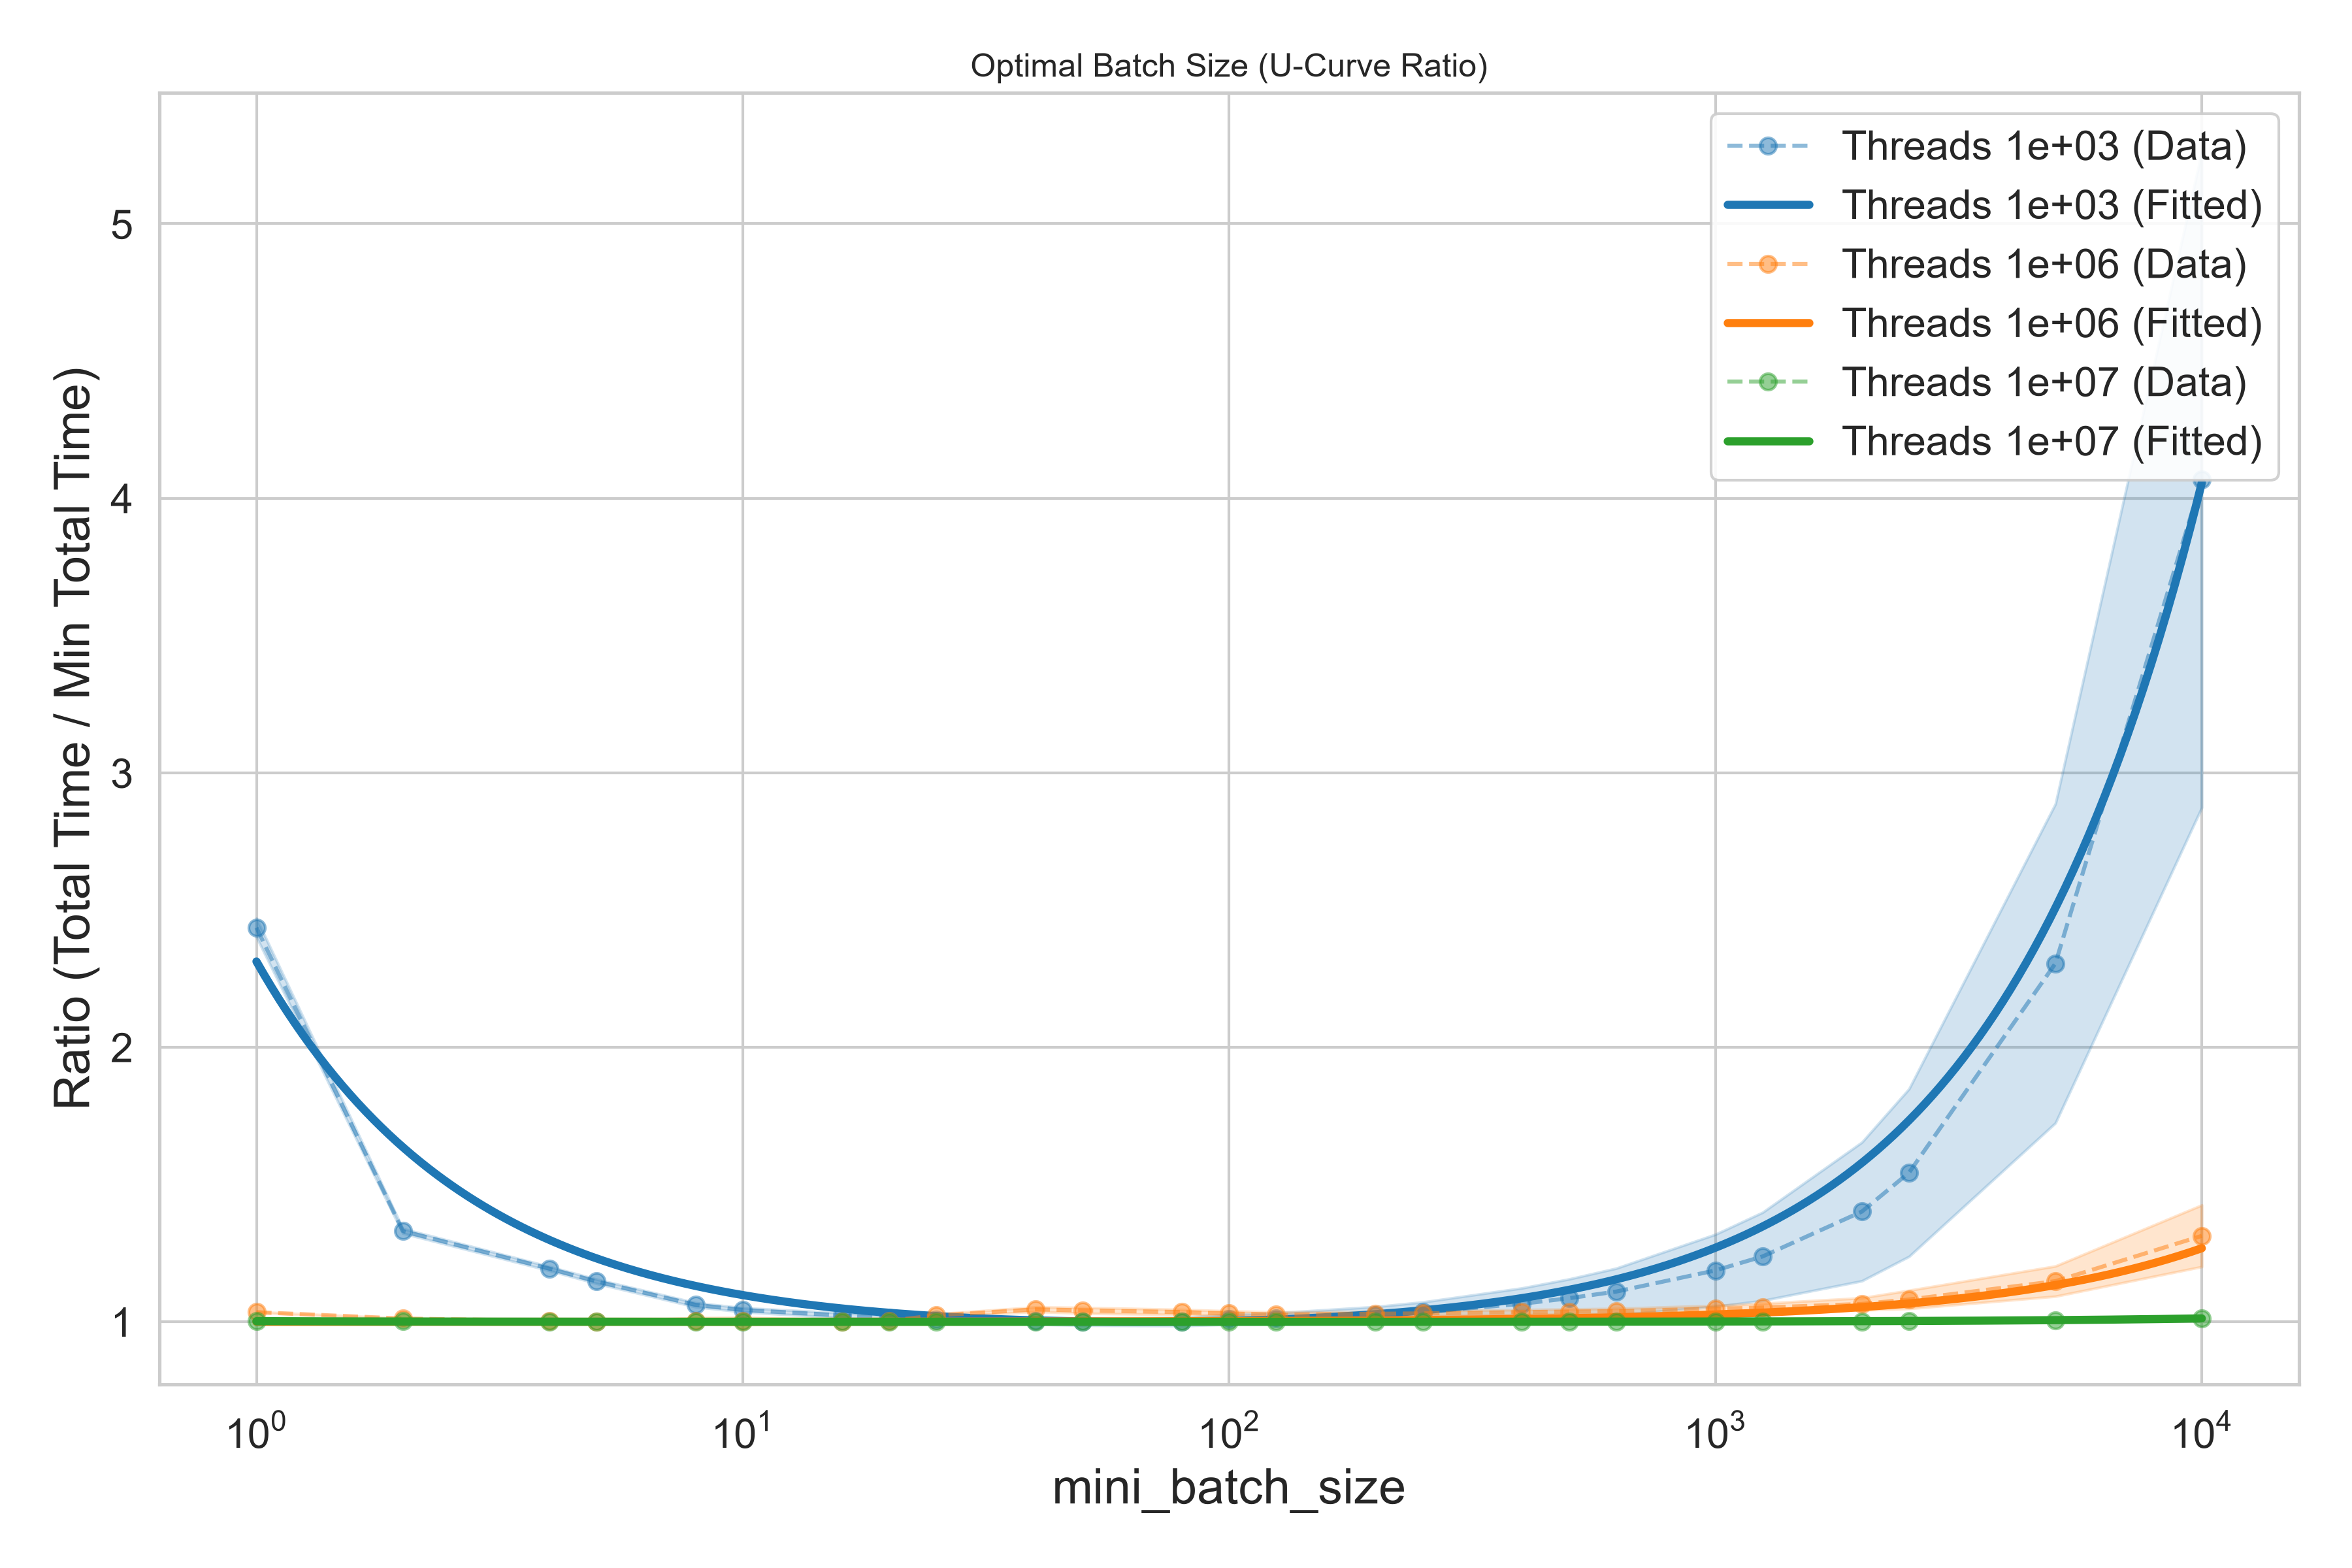
\includegraphics[height=0.7\textheight,width=\textwidth,keepaspectratio]{../assets/3070/figure_4.png}
        \caption{Normalized Execution Time vs Batch Size for Config A (RTX 3070)}
    \end{figure}
\end{frame}

\begin{frame}{Results}{Optimal Batch Size (GTX 1060)}
    \begin{figure}
        \centering
        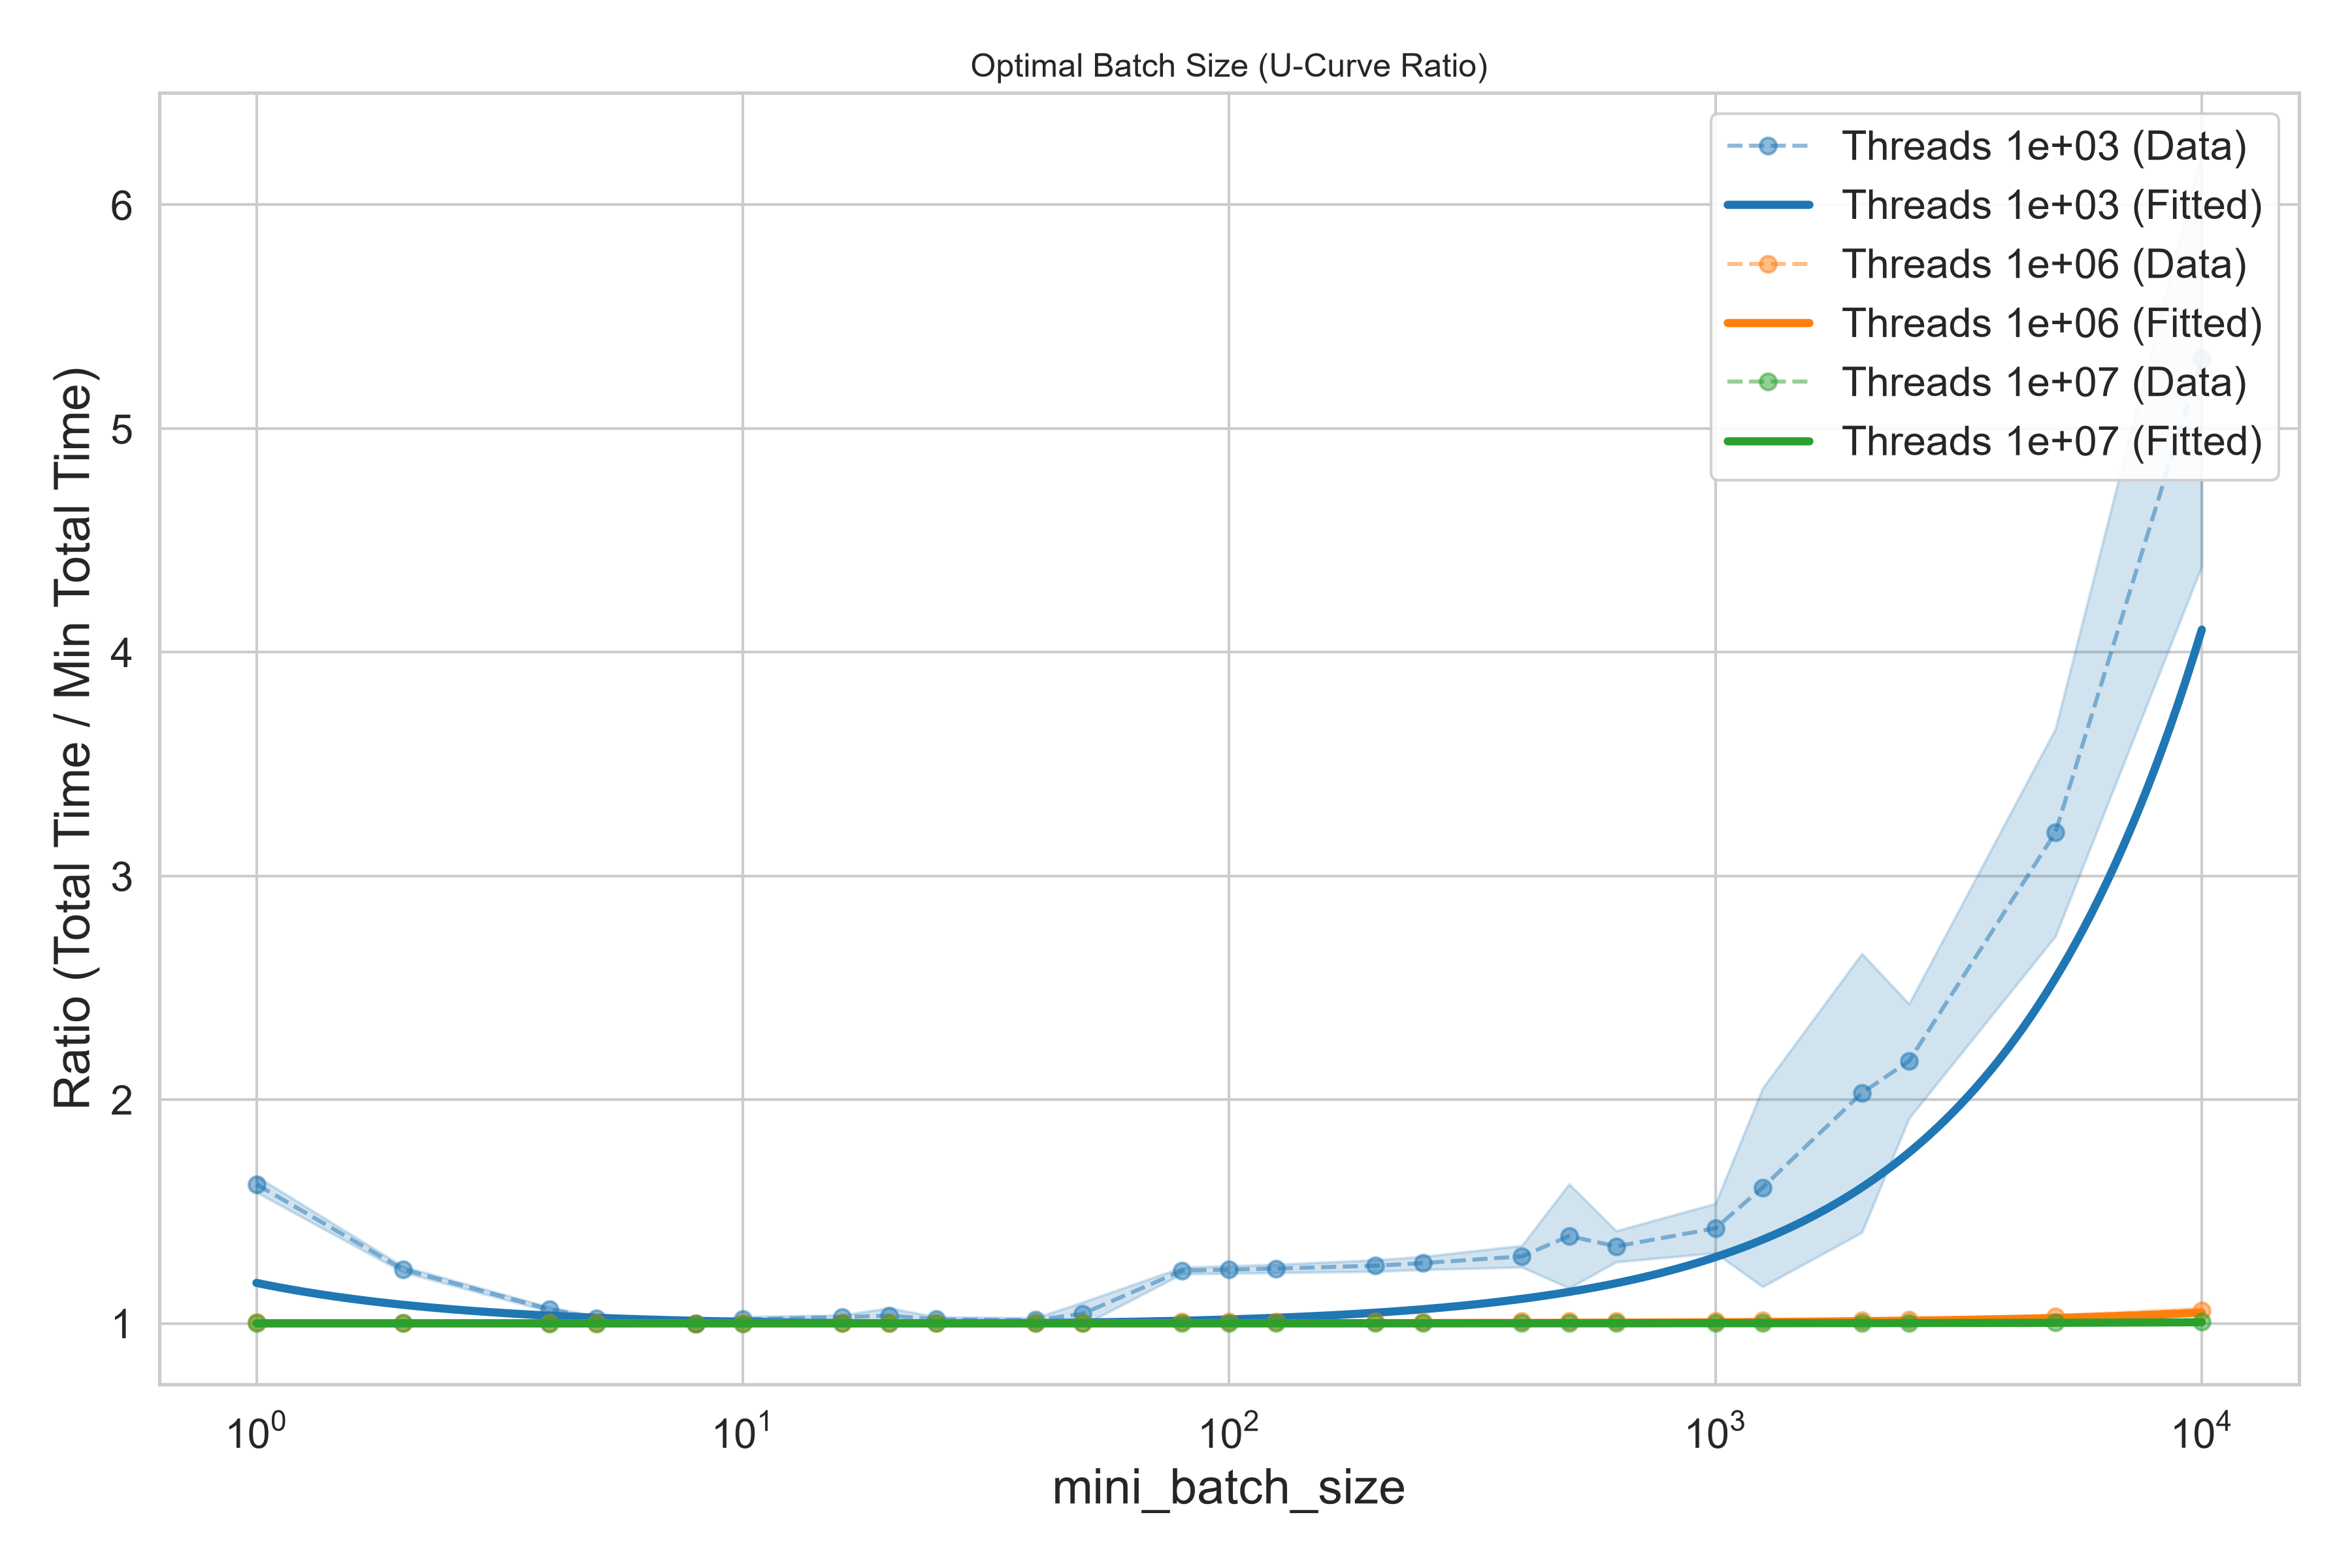
\includegraphics[height=0.7\textheight,width=\textwidth,keepaspectratio]{../assets/1060/figure_4.png}
        \caption{Normalized Execution Time vs Batch Size for Config B (GTX 1060)}
    \end{figure}
\end{frame}

\begin{frame}{Results}{Optimal Batch Size (Tesla T4)}
    \begin{figure}
        \centering
        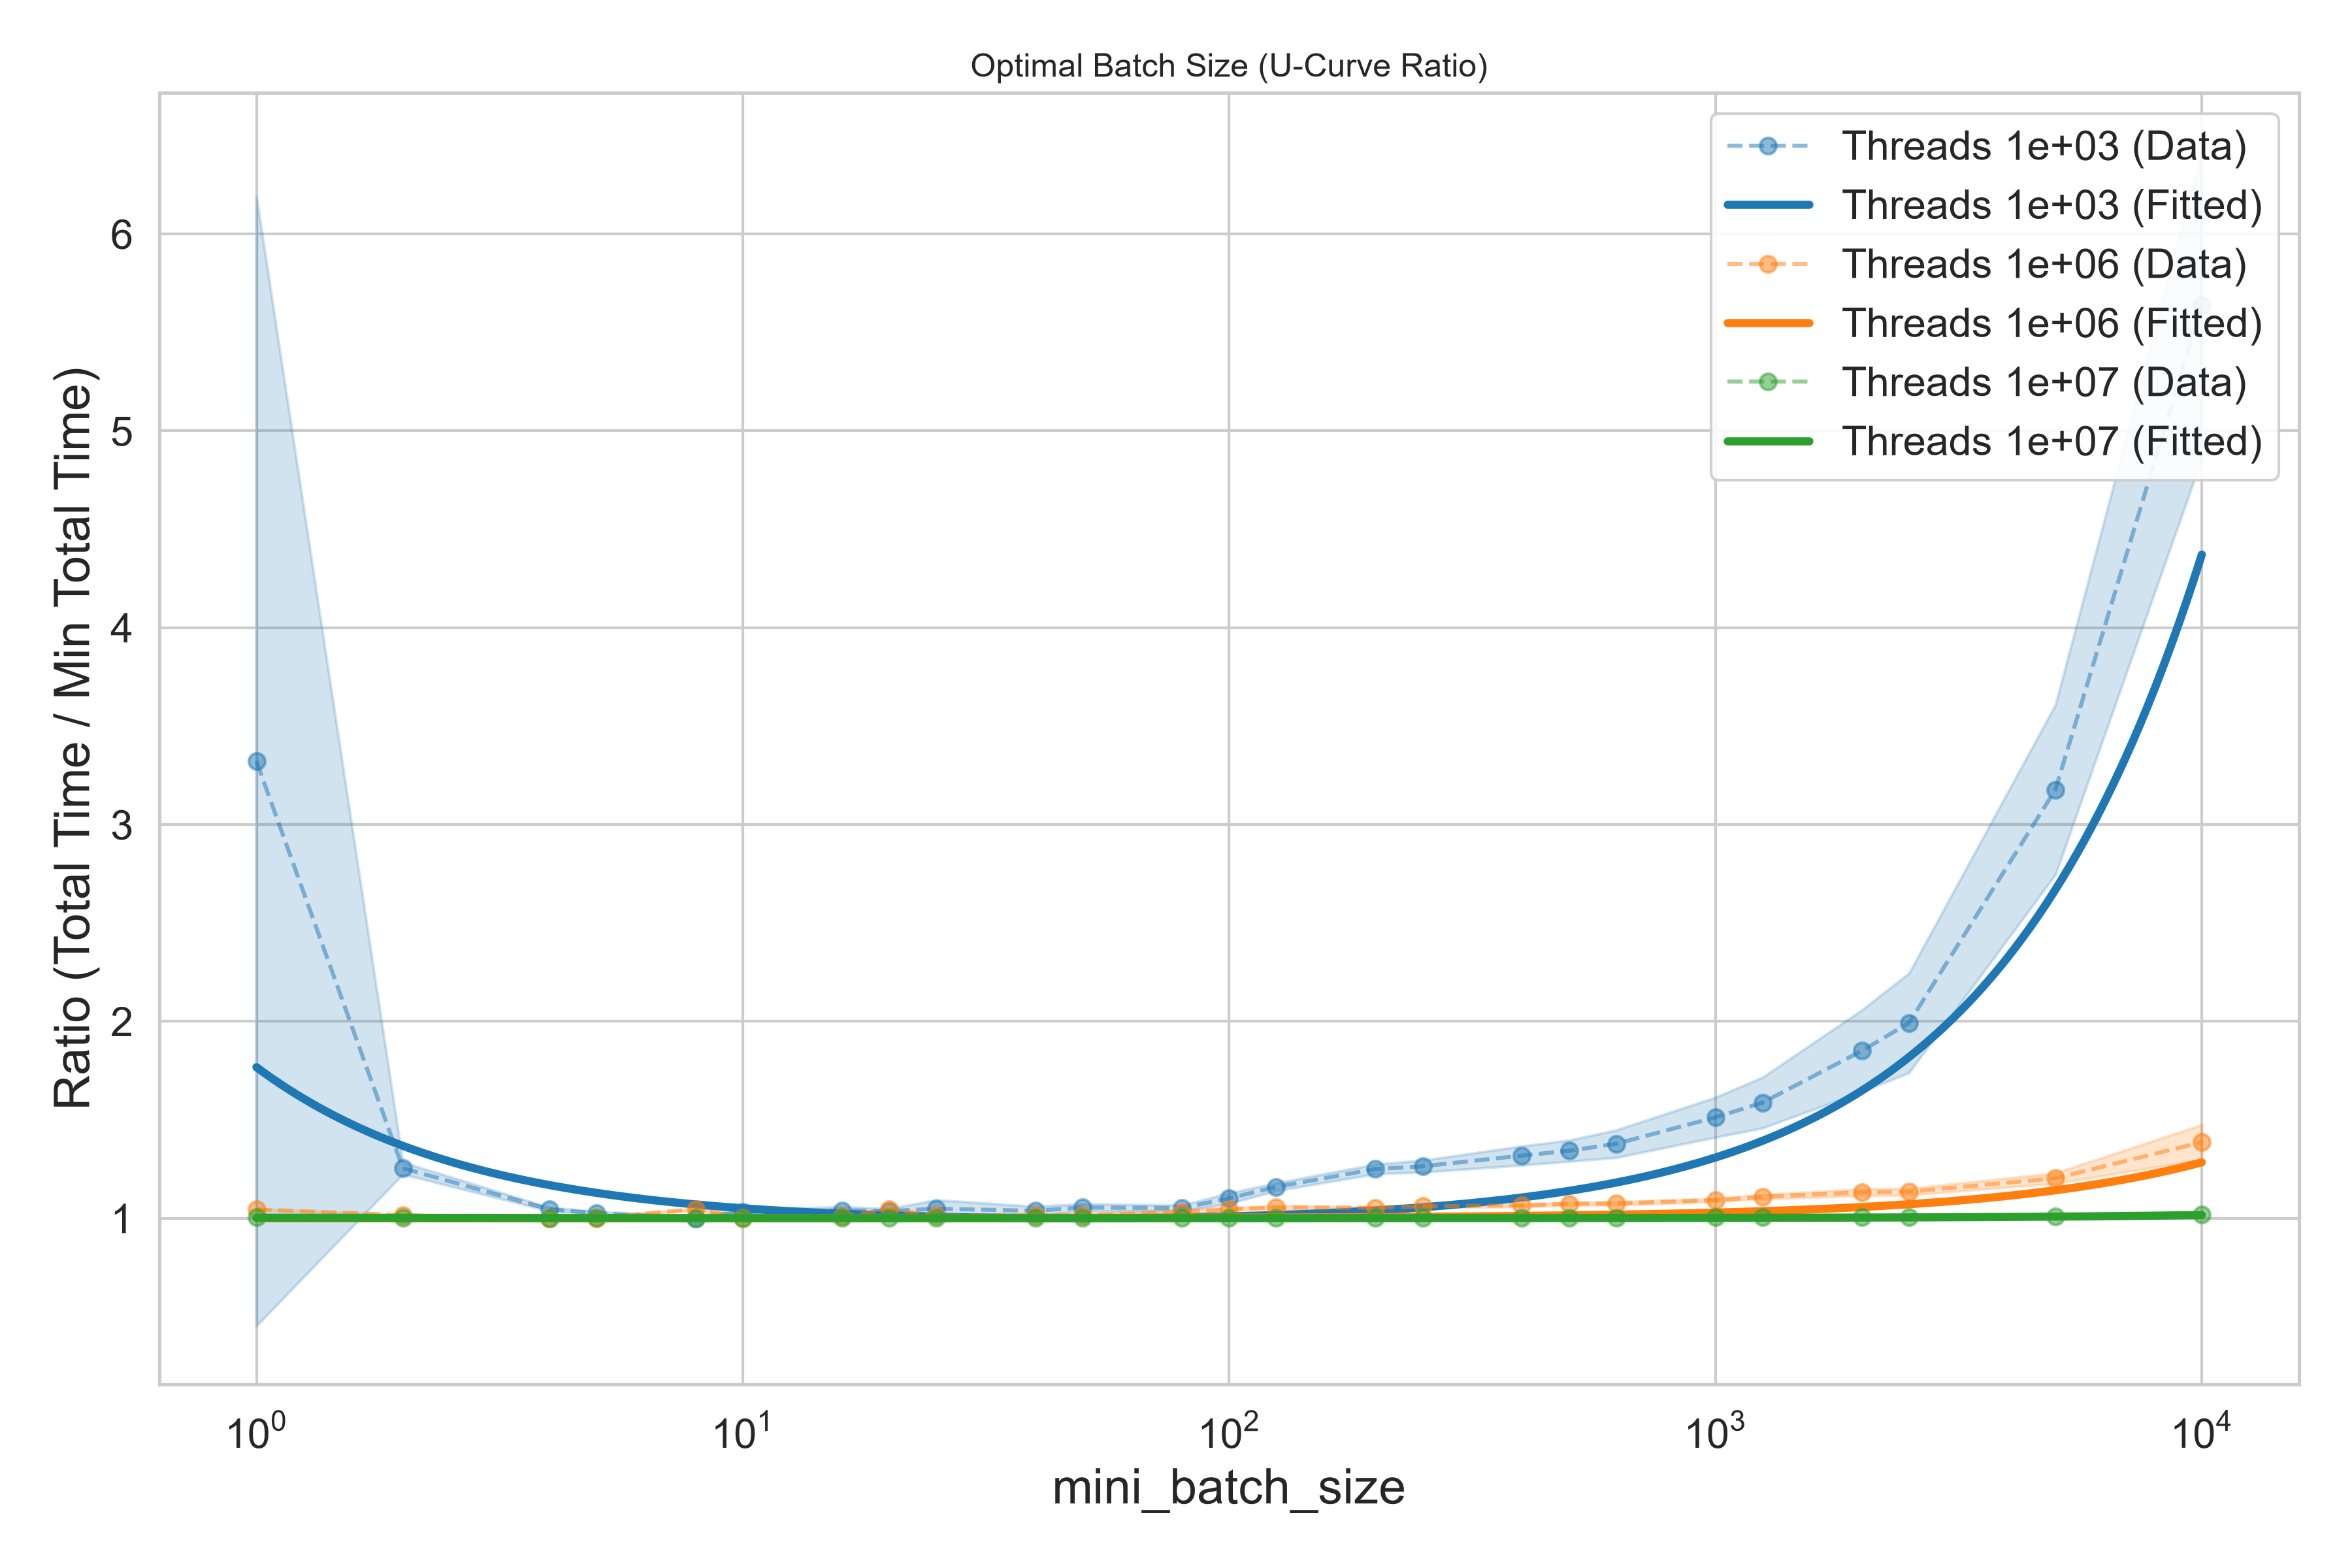
\includegraphics[height=0.7\textheight,width=\textwidth,keepaspectratio]{../assets/t4/figure_4.png}
        \caption{Normalized Execution Time vs Batch Size for Config C (Tesla T4)}
    \end{figure}
\end{frame}

\begin{frame}{Results}{Optimal Batch Size (Original Paper)}
    \begin{figure}
        \centering
        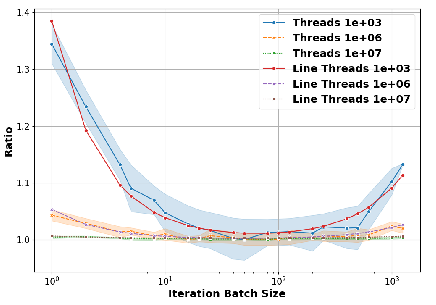
\includegraphics[height=0.7\textheight,width=\textwidth,keepaspectratio]{../article/figures/figure_4.pdf}
        \caption{Normalized Execution Time vs Batch Size (Original Results)}
    \end{figure}
\end{frame}

\begin{frame}{Results}{Optimal Batch Size Insights}
    The "U-shaped" curve clearly validates the 50-100 nodes range for light workloads. For $10^6$ and $10^7$, the execution ratio remains flat (graph size is negligible for heavy workloads).
\end{frame}

\begin{frame}{Results}{Optimal Batch Size Fitting (RTX 3070)}
    \begin{table}
        \centering
        \caption{Fitting parameters for Total Execution Time ($T_{tot} = a \cdot S + b/S + C$)}
        \renewcommand{\arraystretch}{1.2}
        \resizebox{\columnwidth}{!}{%
        \begin{tabular}{rcccccc}
            \toprule
            \textbf{Workload} & \textbf{\(a\)} & \textbf{\(b\)} & \textbf{\(C\)} & \textbf{MAE} & \textbf{\(S_{opt}\) (theo)} & \textbf{\(S_{opt}\) (emp)} \\
            \midrule
            \(10^3\) & $2.64 \times 10^{-6}$ & $1.16 \times 10^{-2}$ & $8.19 \times 10^{-3}$ & $5.55 \times 10^{-4}$ & 66.10 & 50 \\
            \(10^6\) & $2.64 \times 10^{-6}$ & $1.89 \times 10^{-6}$ & $9.84 \times 10^{-2}$ & $1.03 \times 10^{-3}$ & 0.85 & 16 \\
            \(10^7\) & $2.59 \times 10^{-6}$ & $5.21 \times 10^{-3}$ & $2.05 \times 10^{0}$ & $6.01 \times 10^{-4}$ & 44.88 & 80 \\
            \bottomrule
        \end{tabular}%
        }
    \end{table}
\end{frame}

\begin{frame}{Results}{Speed-up Relative to Baseline (RTX 3070)}
    \begin{figure}
        \centering
        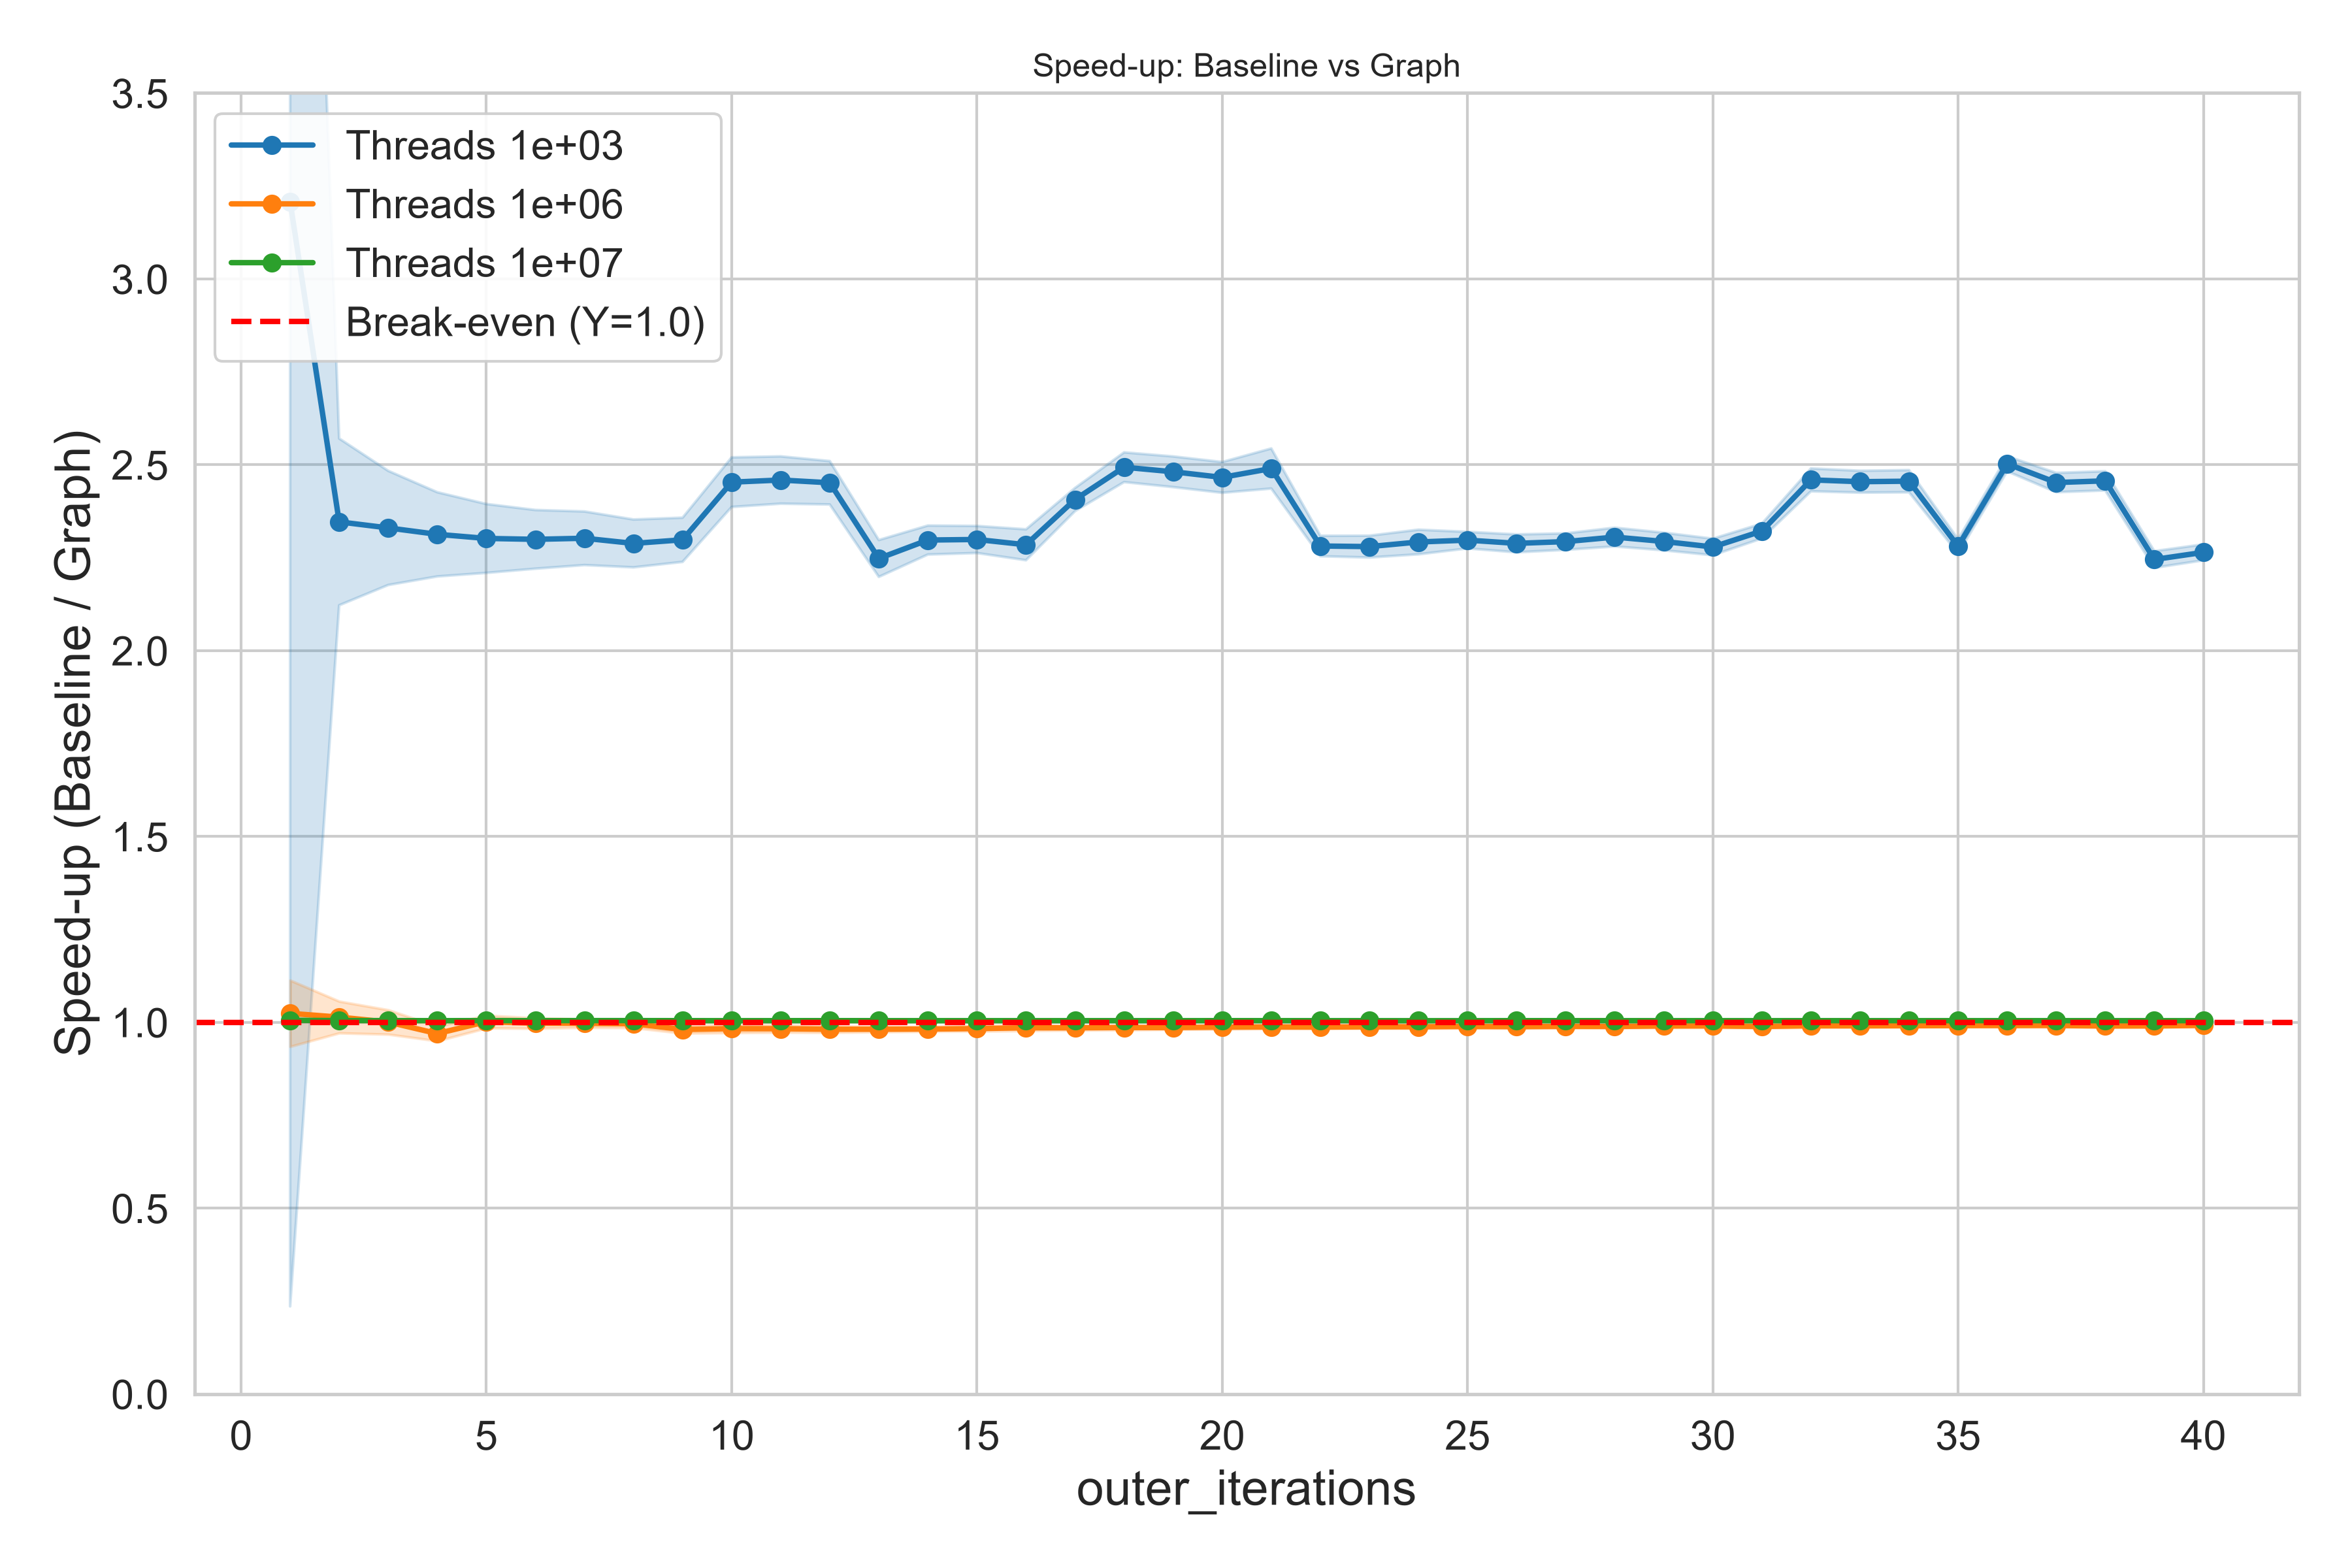
\includegraphics[height=0.7\textheight,width=\textwidth,keepaspectratio]{../assets/3070/figure_6.png}
        \caption{Speed-up of the Unrolling Strategy for Config A (RTX 3070)}
    \end{figure}
\end{frame}

\begin{frame}{Results}{Speed-up Relative to Baseline (GTX 1060)}
    \begin{figure}
        \centering
        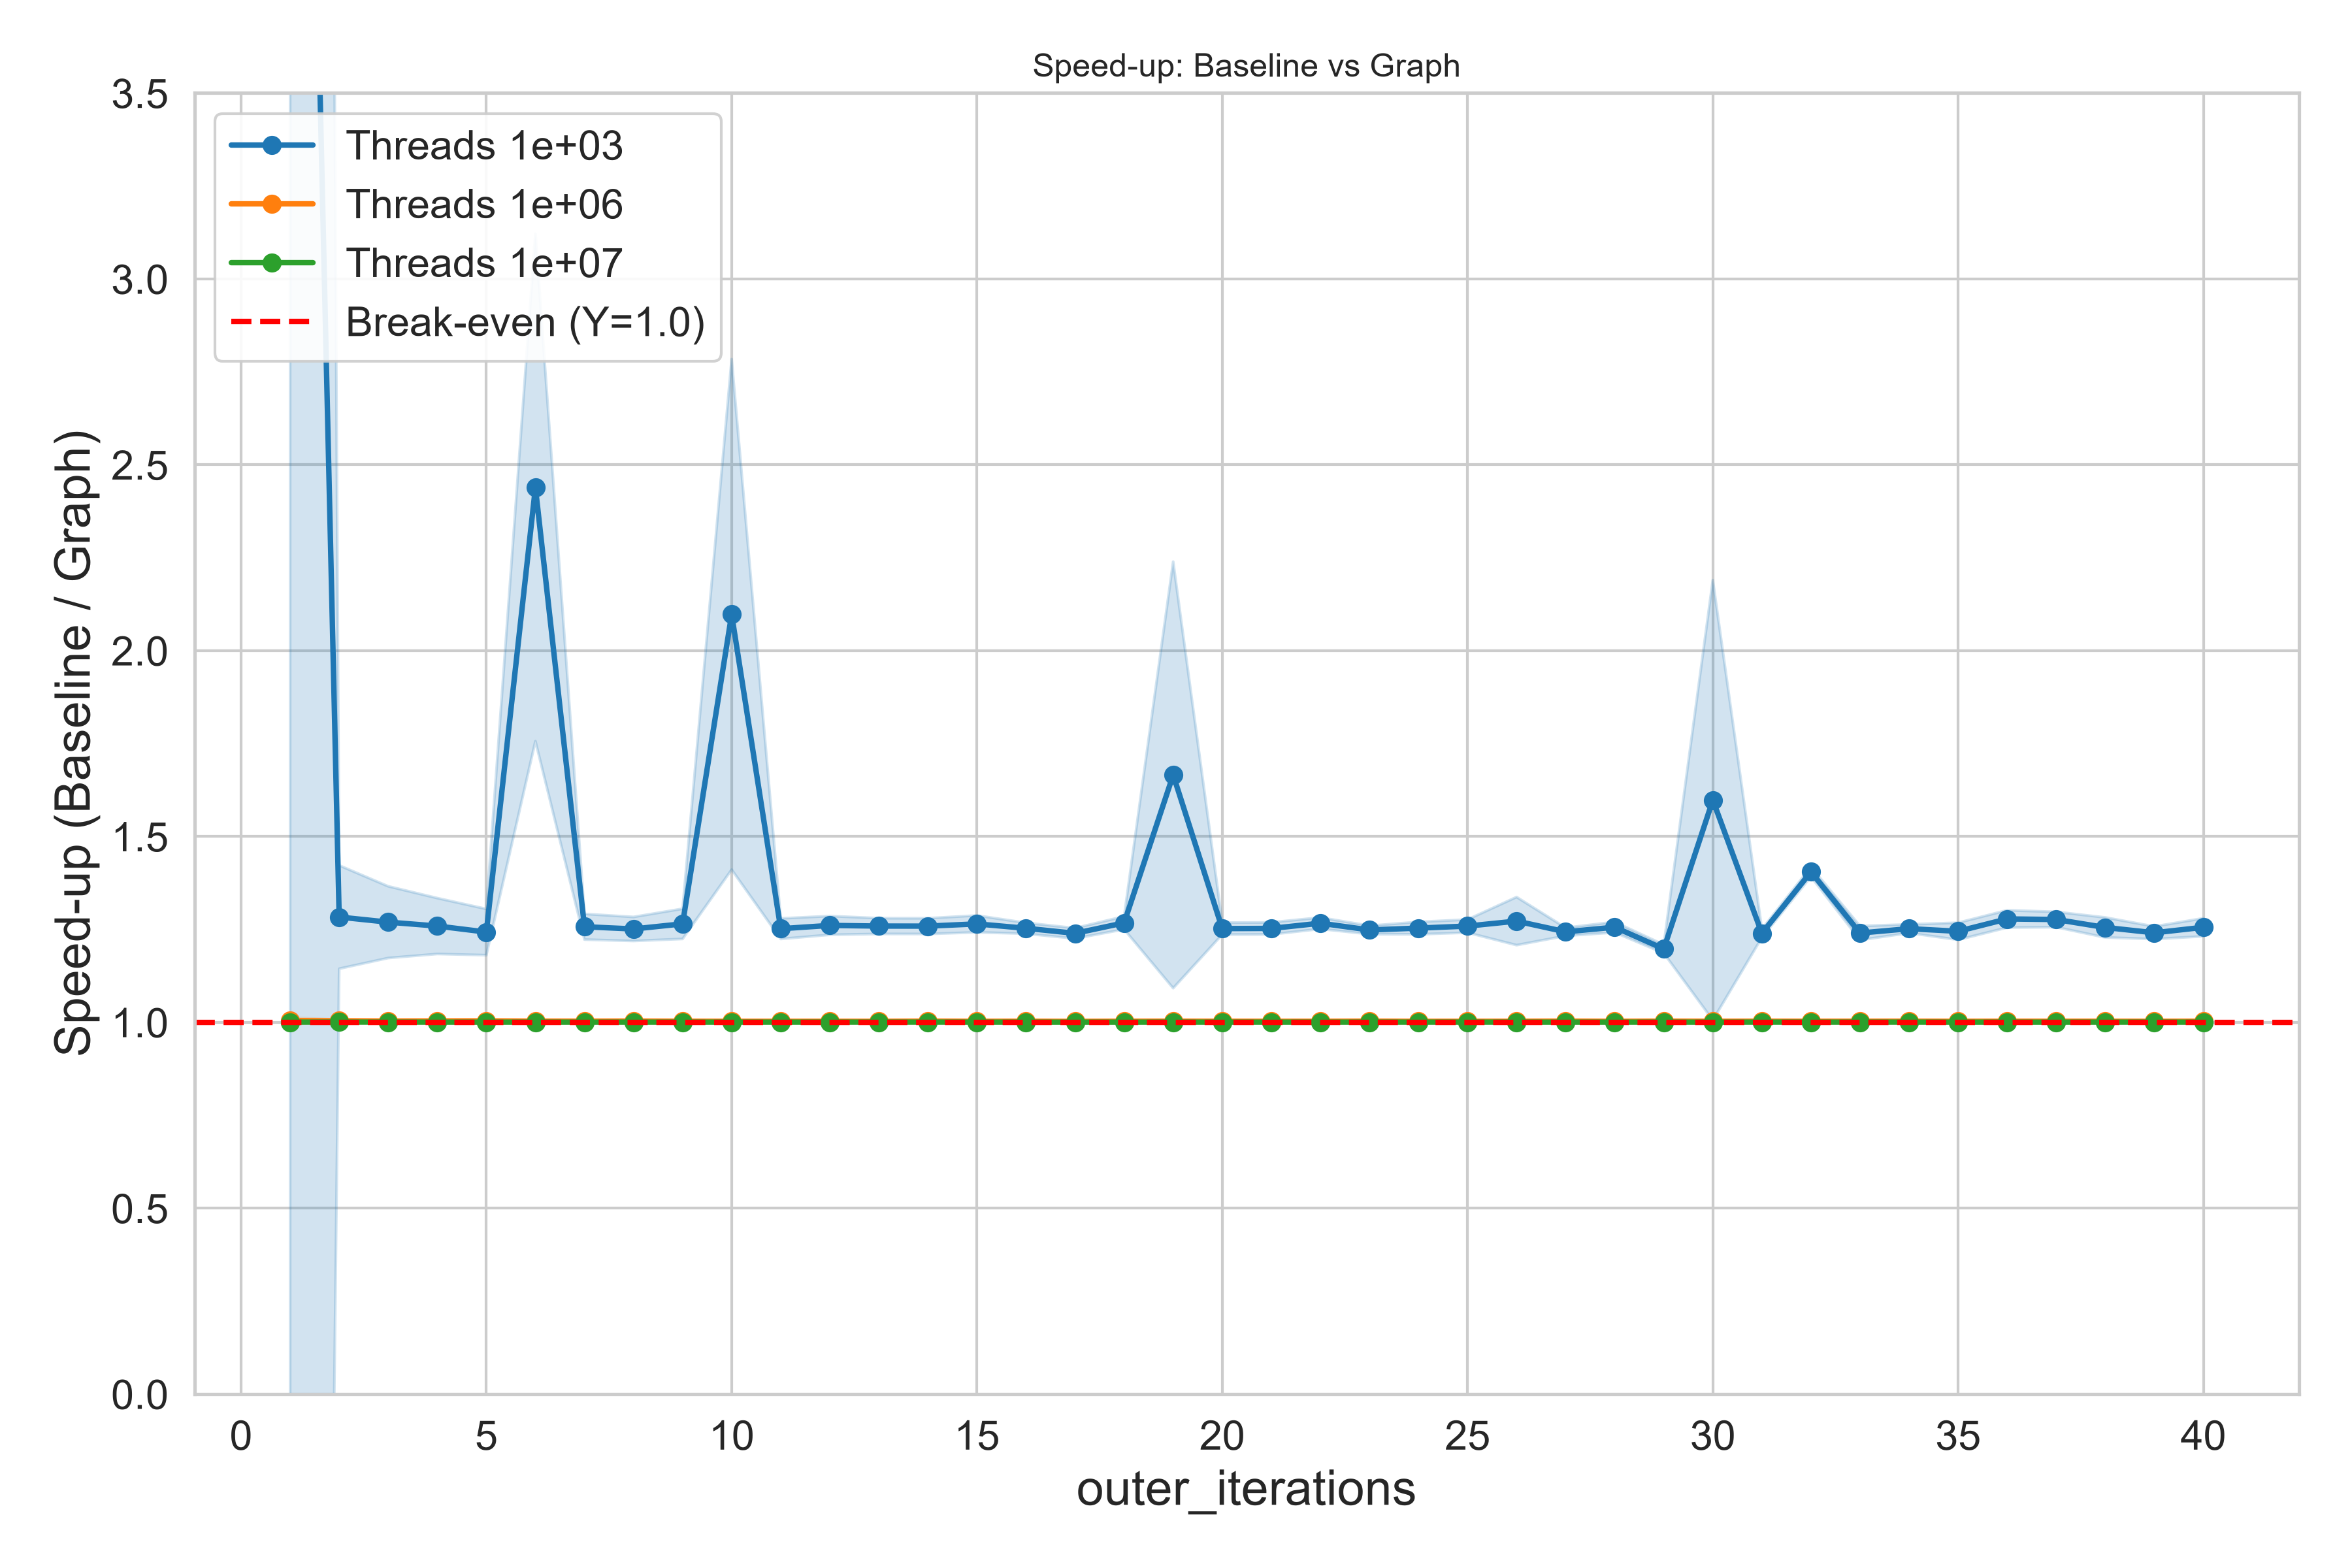
\includegraphics[height=0.7\textheight,width=\textwidth,keepaspectratio]{../assets/1060/figure_6.png}
        \caption{Speed-up of the Unrolling Strategy for Config B (GTX 1060)}
    \end{figure}
\end{frame}

\begin{frame}{Results}{Speed-up Relative to Baseline (Tesla T4)}
    \begin{figure}
        \centering
        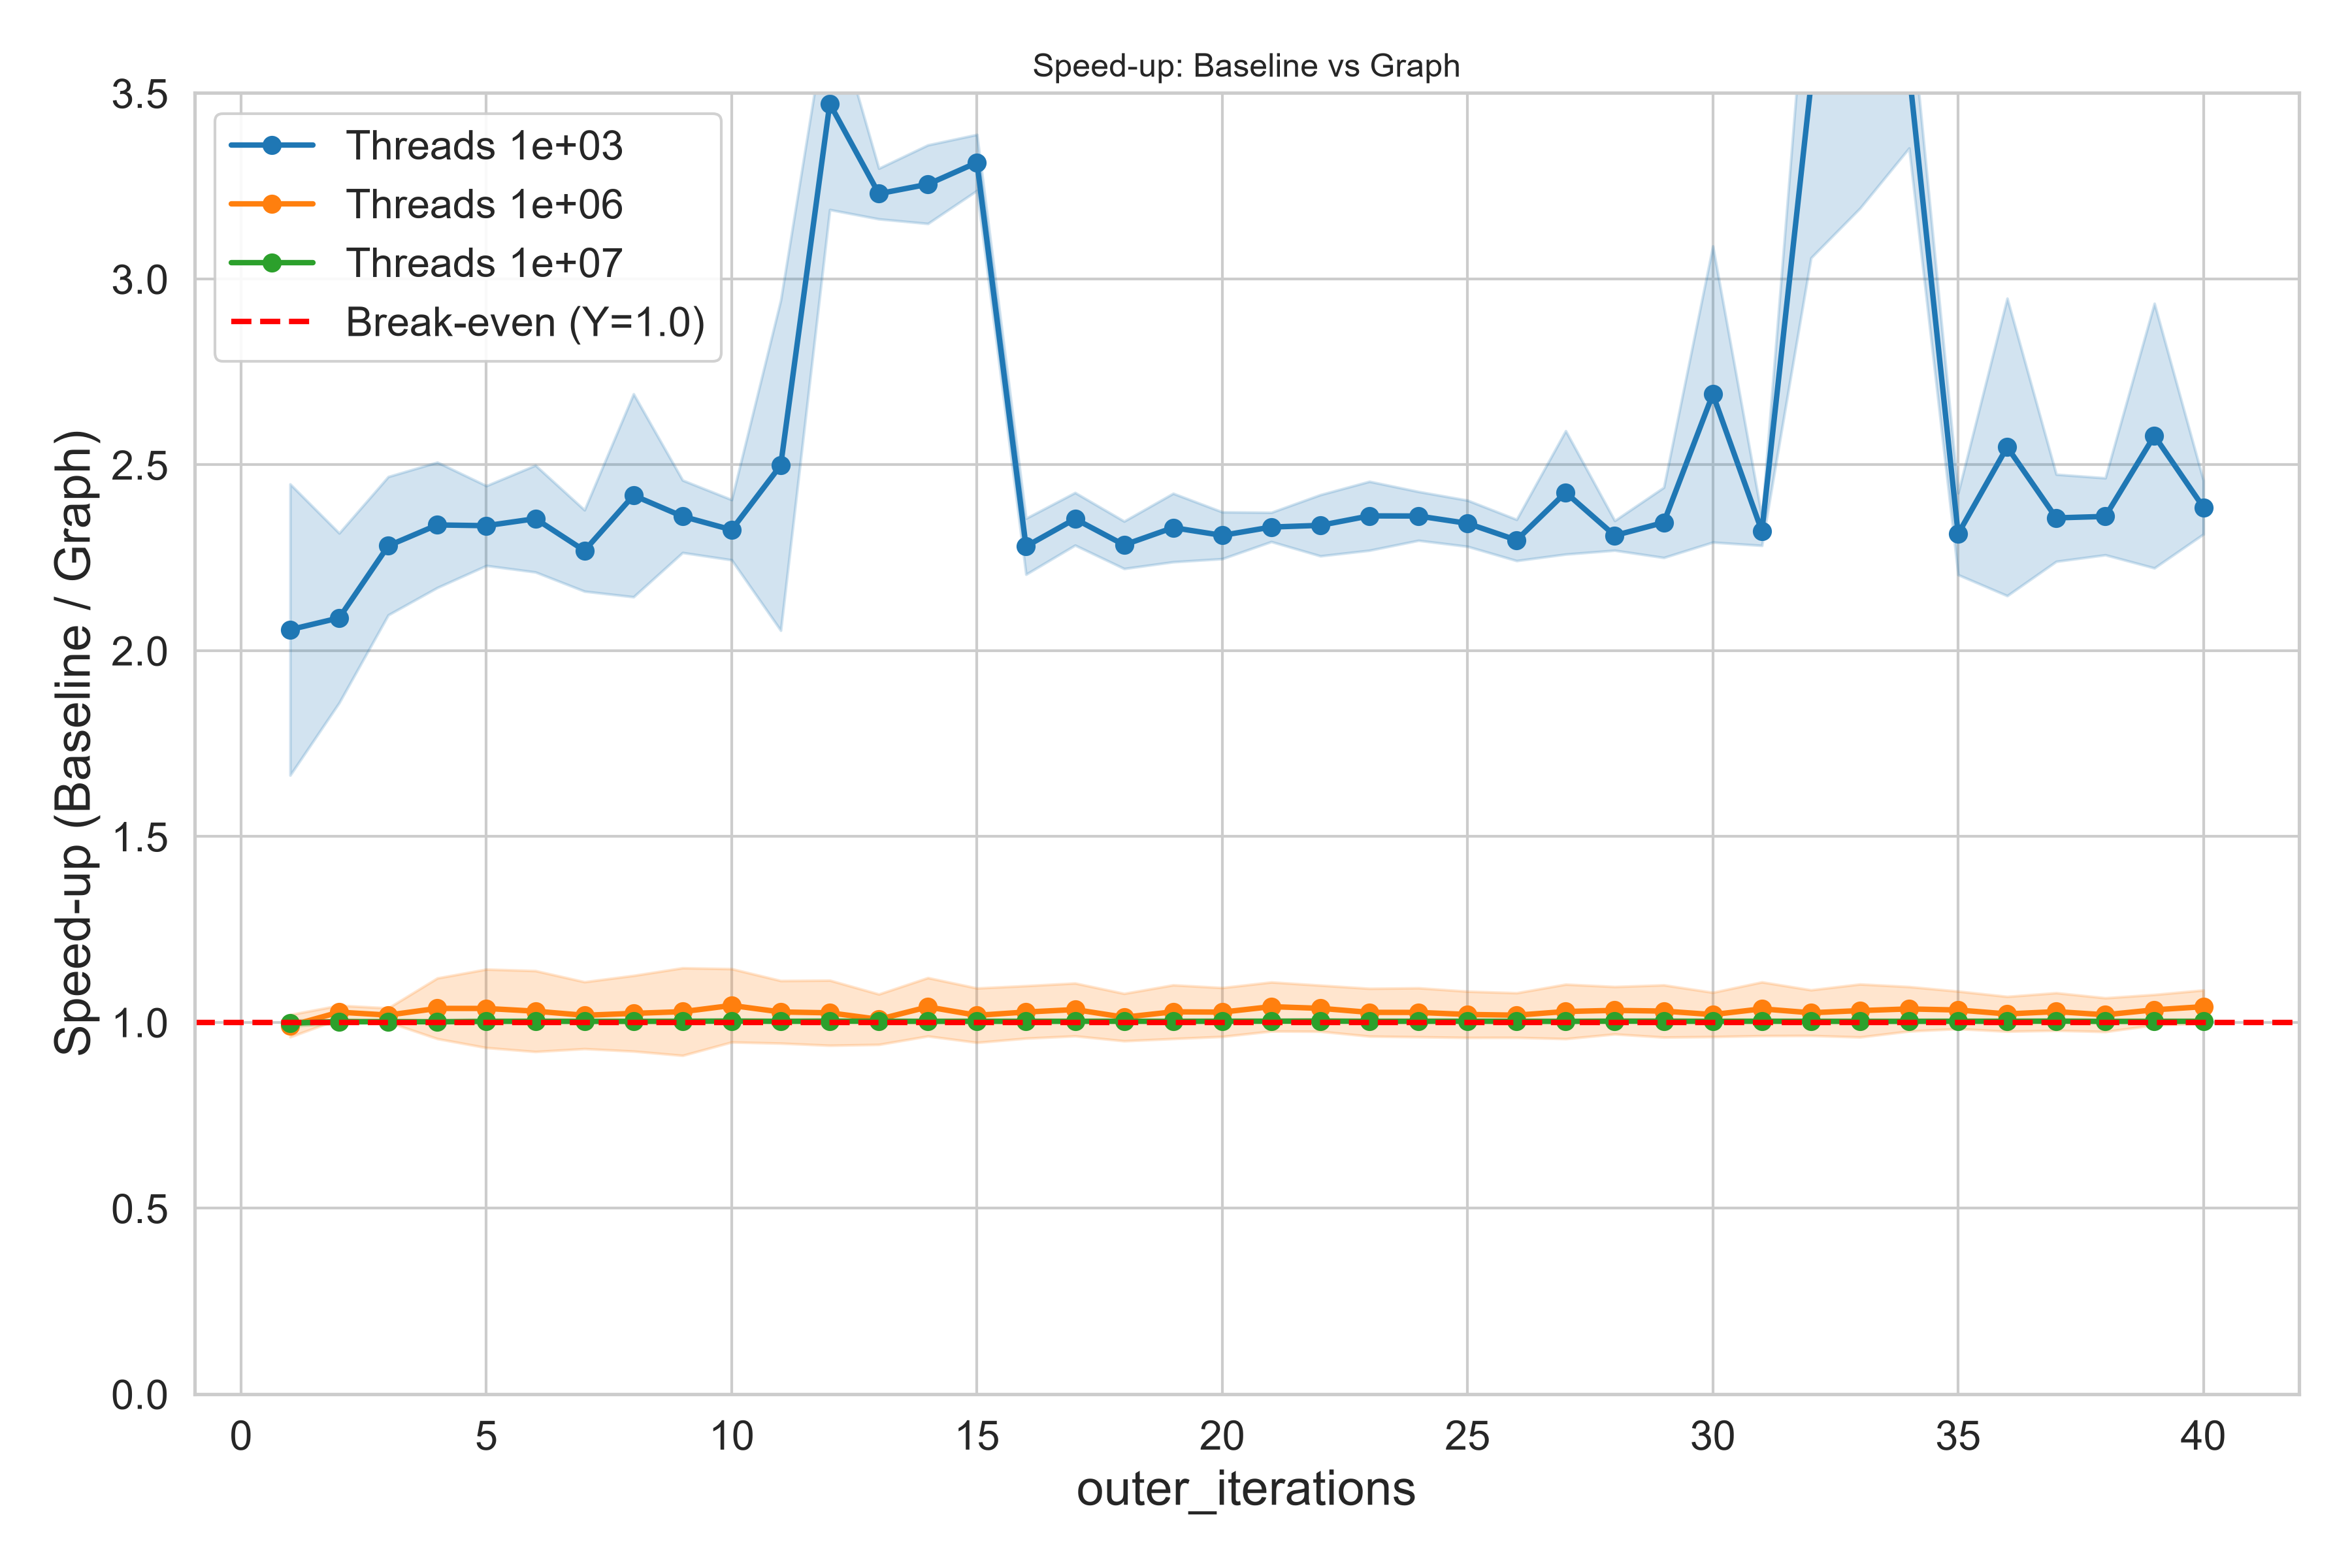
\includegraphics[height=0.7\textheight,width=\textwidth,keepaspectratio]{../assets/t4/figure_6.png}
        \caption{Speed-up of the Unrolling Strategy for Config C (Tesla T4)}
    \end{figure}
\end{frame}

\begin{frame}{Results}{Speed-up Relative to Baseline (Original Paper)}
    \begin{figure}
        \centering
        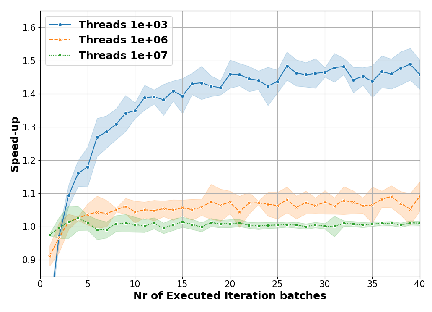
\includegraphics[height=0.7\textheight,width=\textwidth,keepaspectratio]{../article/figures/figure_6.pdf}
        \caption{Speed-up of the Unrolling Strategy (Original Results)}
    \end{figure}
\end{frame}

\begin{frame}{Results}{Speed-up Insights}
    \begin{itemize}
        \item \textbf{Light Workloads}: Original paper reported 1.4x-1.5x speed-up. We observed a dramatically higher speed-up stabilizing between \textbf{2.3x and 2.5x}.
        \item This is likely due to the \textbf{much higher host-device latency} of our tested configurations compared to the authors' A100 and AMD EPYC setup.
        \item \textbf{Heavy Workloads}: Reaches the "break-even" point (exactly 1.0x). Kernel execution time completely dominates launch overhead, yielding neither benefits nor penalties.
    \end{itemize}
\end{frame}

% ---------------------------------------------------------------
\section{Conclusion}
% ---------------------------------------------------------------
\begin{frame}{Conclusion}
    \begin{itemize}
        \item \textbf{Model Validated}: CUDA Graphs for iterative loops are highly effective (inter-kernel latency $T_i$ is strictly lower than launch overhead $T_a$).
        \item \textbf{Hardware Dependency}: Tangible benefits depend heavily on execution environment. This technique is more powerful on configurations with high CPU-to-GPU latency, making it \textbf{very advantageous for older computing systems}.
        \item \textbf{Software Resilience}: Newer driver/CUDA Toolkit versions show greater resilience at larger node counts and reduced memory footprints.
    \end{itemize}
\end{frame}

\begin{frame}[t,allowframebreaks]
    \frametitle{Bibliography}
    \printbibliography[heading=none]
\end{frame}

\begin{frame}[plain,noframenumbering]
	\standoutpage{\bfseries\huge Thank you for your time!}
\end{frame}

\end{document}